\documentclass[]{book}
\usepackage{lmodern}
\usepackage{amssymb,amsmath}
\usepackage{ifxetex,ifluatex}
\usepackage{fixltx2e} % provides \textsubscript
\ifnum 0\ifxetex 1\fi\ifluatex 1\fi=0 % if pdftex
  \usepackage[T1]{fontenc}
  \usepackage[utf8]{inputenc}
\else % if luatex or xelatex
  \ifxetex
    \usepackage{mathspec}
  \else
    \usepackage{fontspec}
  \fi
  \defaultfontfeatures{Ligatures=TeX,Scale=MatchLowercase}
\fi
% use upquote if available, for straight quotes in verbatim environments
\IfFileExists{upquote.sty}{\usepackage{upquote}}{}
% use microtype if available
\IfFileExists{microtype.sty}{%
\usepackage{microtype}
\UseMicrotypeSet[protrusion]{basicmath} % disable protrusion for tt fonts
}{}
\usepackage{hyperref}
\hypersetup{unicode=true,
            pdftitle={Apostila: introdução ao pacote dplyr},
            pdfauthor={Me. Elisângela C. Biazatti Douglas Vinícius Jossivana Macedo},
            pdfborder={0 0 0},
            breaklinks=true}
\urlstyle{same}  % don't use monospace font for urls
\usepackage{natbib}
\bibliographystyle{apalike}
\usepackage{color}
\usepackage{fancyvrb}
\newcommand{\VerbBar}{|}
\newcommand{\VERB}{\Verb[commandchars=\\\{\}]}
\DefineVerbatimEnvironment{Highlighting}{Verbatim}{commandchars=\\\{\}}
% Add ',fontsize=\small' for more characters per line
\usepackage{framed}
\definecolor{shadecolor}{RGB}{248,248,248}
\newenvironment{Shaded}{\begin{snugshade}}{\end{snugshade}}
\newcommand{\AlertTok}[1]{\textcolor[rgb]{0.94,0.16,0.16}{#1}}
\newcommand{\AnnotationTok}[1]{\textcolor[rgb]{0.56,0.35,0.01}{\textbf{\textit{#1}}}}
\newcommand{\AttributeTok}[1]{\textcolor[rgb]{0.77,0.63,0.00}{#1}}
\newcommand{\BaseNTok}[1]{\textcolor[rgb]{0.00,0.00,0.81}{#1}}
\newcommand{\BuiltInTok}[1]{#1}
\newcommand{\CharTok}[1]{\textcolor[rgb]{0.31,0.60,0.02}{#1}}
\newcommand{\CommentTok}[1]{\textcolor[rgb]{0.56,0.35,0.01}{\textit{#1}}}
\newcommand{\CommentVarTok}[1]{\textcolor[rgb]{0.56,0.35,0.01}{\textbf{\textit{#1}}}}
\newcommand{\ConstantTok}[1]{\textcolor[rgb]{0.00,0.00,0.00}{#1}}
\newcommand{\ControlFlowTok}[1]{\textcolor[rgb]{0.13,0.29,0.53}{\textbf{#1}}}
\newcommand{\DataTypeTok}[1]{\textcolor[rgb]{0.13,0.29,0.53}{#1}}
\newcommand{\DecValTok}[1]{\textcolor[rgb]{0.00,0.00,0.81}{#1}}
\newcommand{\DocumentationTok}[1]{\textcolor[rgb]{0.56,0.35,0.01}{\textbf{\textit{#1}}}}
\newcommand{\ErrorTok}[1]{\textcolor[rgb]{0.64,0.00,0.00}{\textbf{#1}}}
\newcommand{\ExtensionTok}[1]{#1}
\newcommand{\FloatTok}[1]{\textcolor[rgb]{0.00,0.00,0.81}{#1}}
\newcommand{\FunctionTok}[1]{\textcolor[rgb]{0.00,0.00,0.00}{#1}}
\newcommand{\ImportTok}[1]{#1}
\newcommand{\InformationTok}[1]{\textcolor[rgb]{0.56,0.35,0.01}{\textbf{\textit{#1}}}}
\newcommand{\KeywordTok}[1]{\textcolor[rgb]{0.13,0.29,0.53}{\textbf{#1}}}
\newcommand{\NormalTok}[1]{#1}
\newcommand{\OperatorTok}[1]{\textcolor[rgb]{0.81,0.36,0.00}{\textbf{#1}}}
\newcommand{\OtherTok}[1]{\textcolor[rgb]{0.56,0.35,0.01}{#1}}
\newcommand{\PreprocessorTok}[1]{\textcolor[rgb]{0.56,0.35,0.01}{\textit{#1}}}
\newcommand{\RegionMarkerTok}[1]{#1}
\newcommand{\SpecialCharTok}[1]{\textcolor[rgb]{0.00,0.00,0.00}{#1}}
\newcommand{\SpecialStringTok}[1]{\textcolor[rgb]{0.31,0.60,0.02}{#1}}
\newcommand{\StringTok}[1]{\textcolor[rgb]{0.31,0.60,0.02}{#1}}
\newcommand{\VariableTok}[1]{\textcolor[rgb]{0.00,0.00,0.00}{#1}}
\newcommand{\VerbatimStringTok}[1]{\textcolor[rgb]{0.31,0.60,0.02}{#1}}
\newcommand{\WarningTok}[1]{\textcolor[rgb]{0.56,0.35,0.01}{\textbf{\textit{#1}}}}
\usepackage{longtable,booktabs}
\usepackage{graphicx,grffile}
\makeatletter
\def\maxwidth{\ifdim\Gin@nat@width>\linewidth\linewidth\else\Gin@nat@width\fi}
\def\maxheight{\ifdim\Gin@nat@height>\textheight\textheight\else\Gin@nat@height\fi}
\makeatother
% Scale images if necessary, so that they will not overflow the page
% margins by default, and it is still possible to overwrite the defaults
% using explicit options in \includegraphics[width, height, ...]{}
\setkeys{Gin}{width=\maxwidth,height=\maxheight,keepaspectratio}
\IfFileExists{parskip.sty}{%
\usepackage{parskip}
}{% else
\setlength{\parindent}{0pt}
\setlength{\parskip}{6pt plus 2pt minus 1pt}
}
\setlength{\emergencystretch}{3em}  % prevent overfull lines
\providecommand{\tightlist}{%
  \setlength{\itemsep}{0pt}\setlength{\parskip}{0pt}}
\setcounter{secnumdepth}{5}
% Redefines (sub)paragraphs to behave more like sections
\ifx\paragraph\undefined\else
\let\oldparagraph\paragraph
\renewcommand{\paragraph}[1]{\oldparagraph{#1}\mbox{}}
\fi
\ifx\subparagraph\undefined\else
\let\oldsubparagraph\subparagraph
\renewcommand{\subparagraph}[1]{\oldsubparagraph{#1}\mbox{}}
\fi

%%% Use protect on footnotes to avoid problems with footnotes in titles
\let\rmarkdownfootnote\footnote%
\def\footnote{\protect\rmarkdownfootnote}

%%% Change title format to be more compact
\usepackage{titling}

% Create subtitle command for use in maketitle
\providecommand{\subtitle}[1]{
  \posttitle{
    \begin{center}\large#1\end{center}
    }
}

\setlength{\droptitle}{-2em}

  \title{Apostila: introdução ao pacote dplyr}
    \pretitle{\vspace{\droptitle}\centering\huge}
  \posttitle{\par}
    \author{Me. Elisângela C. BiazattiDouglas ViníciusJossivana Macedo}
    \preauthor{\centering\large\emph}
  \postauthor{\par}
      \predate{\centering\large\emph}
  \postdate{\par}
    \date{22 de outubro de 2019}

\usepackage{booktabs}

\begin{document}
\maketitle

{
\pagestyle{empty}
\begin{titlepage}
   \begin{center}

       \Huge

       \textbf{Title}

       \vspace{0.5cm}

       \LARGE
       \textbf{Subtitle}

   \end{center}
\end{titlepage}

\begin{titlepage}
   \begin{center}

       \Huge

       \textbf{AnotherTitle}

       \vspace{0.5cm}

       \LARGE
       \textbf{Subtitle}

   \end{center}
\end{titlepage}
}

{
\setcounter{tocdepth}{1}
\tableofcontents
}
\hypertarget{prefuxe1cio}{%
\chapter{Prefácio}\label{prefuxe1cio}}

\begin{center}
\includegraphics[width=0.3\linewidth]{imagens/dplyr} \end{center}

Este material foi elaborado com o proprósito de um minicurso, que tem como objetivo apresentar algumas ideias das funções básicas do pacote \texttt{dplyr}. Este material baseou-se em vários em livros, podemos usar um computador e um pouco de criatividade para explorar essas idéias em uma variedade de situações. Usamos R com o RStudio para fazer todo o nosso trabalho.

O livro \href{https://r4ds.had.co.nz/}{R for data science} é o mais indicado para aprender sobre o universo \texttt{tidyverse}. Foi usado o livro do Roger D. Peng \href{https://bookdown.org/rdpeng/rprogdatascience/}{R Programming for Data Science} essencial para compreender as noções básicas do R. Nesse minicurso abordamos mais sobre a gramática das funções básicas do \texttt{dplyr} alguns exemplos e exercícios abordados.

\hypertarget{puxfablico-alvo}{%
\section{Público-alvo}\label{puxfablico-alvo}}

\begin{itemize}
\tightlist
\item
  Estudantes de estatística que desejam ganhar tempo nos trabalhos da faculdade;
\item
  Acadêmicos com interesse em aprender análises e códigos mais legíveis em R.
\end{itemize}

\hypertarget{conteuxfado}{%
\section{Conteúdo:}\label{conteuxfado}}

\begin{verbatim}
- Primeiro dia (22/10): Breve introdução ao R, Tibbles e Data frames,
tidyr, exercícios; 
- Segundo dia (23/10): select(), rename(), arrange(), 
mutate(), summarise(), exercícios;
- Terceiro dia (24/10): agrupar dados, combinar conjuntos de dados.
\end{verbatim}

\hypertarget{pruxe9-requisitos}{%
\section{Pré-requisitos}\label{pruxe9-requisitos}}

\hypertarget{intro}{%
\chapter{Introdução}\label{intro}}

\begin{quote}
``Existem apenas dois tipos de idiomas: os que as pessoas reclamam e os que ninguém usa''. - Bjarne Stroustrup
\end{quote}

O modelo típico de análise de dados é similar:

\begin{center}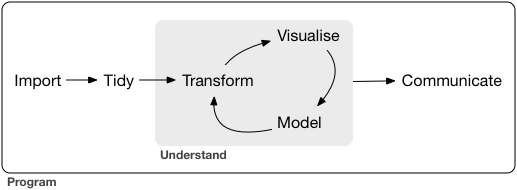
\includegraphics[width=0.75\linewidth]{imagens/data-science} \end{center}

Primeiramente, você deve \textbf{importar} seus dados para o R. Significa que você pega os dados armazenados em um arquivo, banco de dados ou API da Web e carrega-os em um data frames no R.

Logo após, a ideia é \textbf{organizá}-los. Significa armazená-los de forma consistente.

Depois de arrumar os dados, o próximo passo é \textbf{transformá}-los. Significa restringir observações de interesse, criar novas variáveis

Depois de organizar os dados com as variáveis necessárias, existem dois mecanismos principais de geração de conhecimento: visualização e modelagem. Eles têm pontos fortes e fracos complementares, portanto qualquer análise real se repetirá entre eles várias vezes.

A \textbf{visualização} é uma atividade fundamentalmente humana. Uma boa visualização mostrará coisas que você não esperava, ou fará novas perguntas sobre os dados.

\textbf{Modelos} são ferramentas complementares para visualização. Depois de fazer suas perguntas suficientemente precisas, você pode usar um modelo para respondê-las.

O último passo da ciência de dados é a \textbf{comunicação}, uma parte absolutamente crítica de qualquer projeto de análise de dados. Não importa o quão bem seus modelos e visualização levaram você a entender os dados, a menos que você também possa comunicar seus resultados a outras pessoas.

Ao redor de todas essas ferramentas está a programação. A programação é uma ferramenta transversal que você usa em todas as partes do projeto. Você não precisa ser um programador especialista para ser um cientista de dados, mas aprender mais sobre programação compensa, porque se tornar um programador melhor permite automatizar tarefas comuns e resolver novos problemas com maior facilidade.

\hypertarget{universo-tidyverse}{%
\section{\texorpdfstring{Universo \texttt{tidyverse}}{Universo tidyverse}}\label{universo-tidyverse}}

\begin{center}
\includegraphics[width=0.25\linewidth]{imagens/hex-tidyverse} \end{center}

O tidyverse é uma coleção de pacotes R projetados para ciência de dados. Todos os pacotes compartilham uma filosofia de design, gramática e estruturas de dados subjacentes.

Os princípios fundamentais do \texttt{tidyverse} são:

\begin{itemize}
\tightlist
\item
  1.Reutilizar estruturas de dados existentes;
\item
  2.Organizar funções simples usando o pipe;
\item
  3.Aderir à programação funcional;
\item
  4.Projetado para ser usado por seres humanos.
\end{itemize}

Assim como o processo típico do passo a passo apresentando anteriormente para análise de dados, o \texttt{tidyverse} é a ferramenta que o ajuda eficientemente a executar este processo.

\begin{Shaded}
\begin{Highlighting}[]
\KeywordTok{library}\NormalTok{(tidyverse) }\CommentTok{#Carregar o pacote.}
\KeywordTok{tidyverse_logo}\NormalTok{() }\CommentTok{#Logo}
\end{Highlighting}
\end{Shaded}

\begin{verbatim}
## * __  _    __   .    o           *  . 
##  / /_(_)__/ /_ ___  _____ _______ ___ 
## / __/ / _  / // / |/ / -_) __(_-</ -_)
## \__/_/\_,_/\_, /|___/\__/_/ /___/\__/ 
##      *  . /___/      o      .       *
\end{verbatim}

\hypertarget{porque-devo-aprender-r-e-rstudio}{%
\section{Porque devo aprender R e RStudio?}\label{porque-devo-aprender-r-e-rstudio}}

R é uma linguagem de programação estatística que vem passando por diversas evoluções e se tornando cada vez mais uma linguagem de amplos objetivos. Podemos entender o R também como um conjunto de pacotes e ferramentas estatísticas, munido de funções que facilitam sua utilização, desde a criação de simples rotinas até análises de dados complexas, com visualizações bem acabadas.

Segue alguns motivos para aprender o R:

\begin{itemize}
\tightlist
\item
  É completamente gratuito e de livre distribuição;
\item
  Curva de aprendizado bastante amigável, sendo muito fácil de se aprender;
\item
  Enorme quantidade de tutoriais e ajuda disponíveis gratuitamente na internet;
\item
  É excelente para criar rotinas e sistematizar tarefas repetitivas;
\item
  Amplamente utilizado pela comunidade acadêmica e pelo mercado;
\item
  Quantidade enorme de pacotes, para diversos tipos de necessidades;
\item
  Ótima ferramenta para criar relatórios e gráficos.
\end{itemize}

Apenas para exemplificar-se sua versatilidade, esta apostila e os slides das aulas foram todos feitos em R.

A primeira coisa que você precisa fazer para iniciar o R é instalá-lo no seu computador. O R funciona em praticamente todas as plataformas disponíveis, incluindo os sistemas Windows, Mac OS X e Linux amplamente disponíveis.

\begin{itemize}
\tightlist
\item
  Para instalar o R, baixe a versão adequada para seu computador em: \url{https://cloud.r-project.org/}.
\end{itemize}

Uma nova versão principal do R sai uma vez por ano, e há 2 ou 3 versões menores a cada ano. É uma boa ideia atualizar regularmente. A atualização pode ser um pouco complicada, especialmente para as versões principais, que exigem a reinstalação de todos os seus pacotes.

Há também um ambiente de desenvolvimento integrado (IDE) disponível para o R, construído pelo RStudio. IDE, do inglês \textbf{Integrated Development Environment} ou Ambiente de Desenvolvimento Integrado, é um programa de computador que reúne características e ferramentas de apoio ao desenvolvimento de software com o objetivo de agilizar este processo. O RStudio é atualizado duas vezes por ano. Quando uma nova versão estiver disponível, o RStudio informará você.

\begin{itemize}
\tightlist
\item
  Para instalar o RStudio, baixe a versão adequada para seu computador em: \url{https://www.rstudio.com/products/rstudio/download/}.
\end{itemize}

Você pode ver como instalar o R e o RStudio aqui:

\begin{itemize}
\tightlist
\item
  \href{https://www.youtube.com/watch?v=orjLGFmx6l4}{Instalando o RStudio}.
\end{itemize}

Após instalado, o R tem uma interface assim, com apenas o console para digitar comandos:

\begin{center}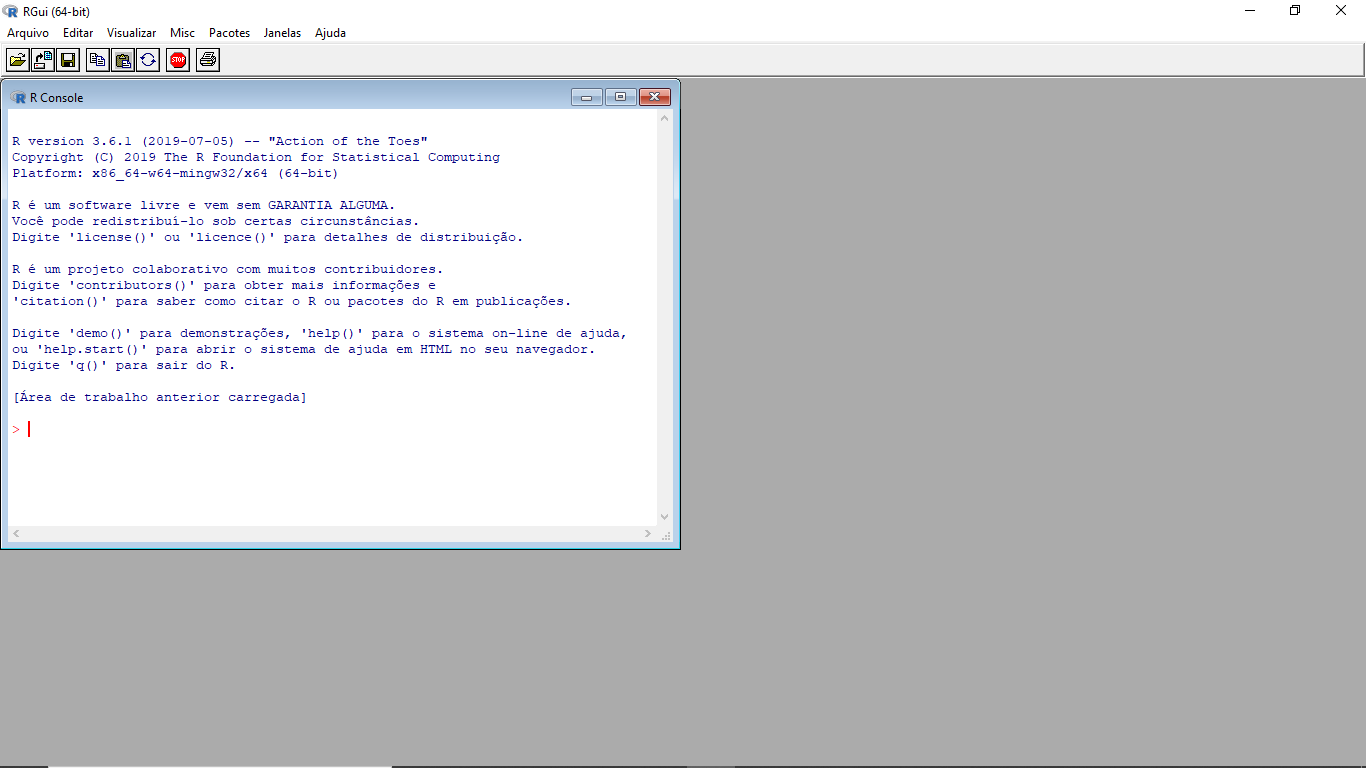
\includegraphics[width=0.9\linewidth]{imagens/r-project} \end{center}

Experimente um comando: 2+2, cujo output é 4:

\begin{Shaded}
\begin{Highlighting}[]
\DecValTok{2} \OperatorTok{+}\StringTok{ }\DecValTok{2}
\end{Highlighting}
\end{Shaded}

\begin{verbatim}
## [1] 4
\end{verbatim}

E a interface do RStudio é dividida, inicialmente, em 3 partes:

\begin{center}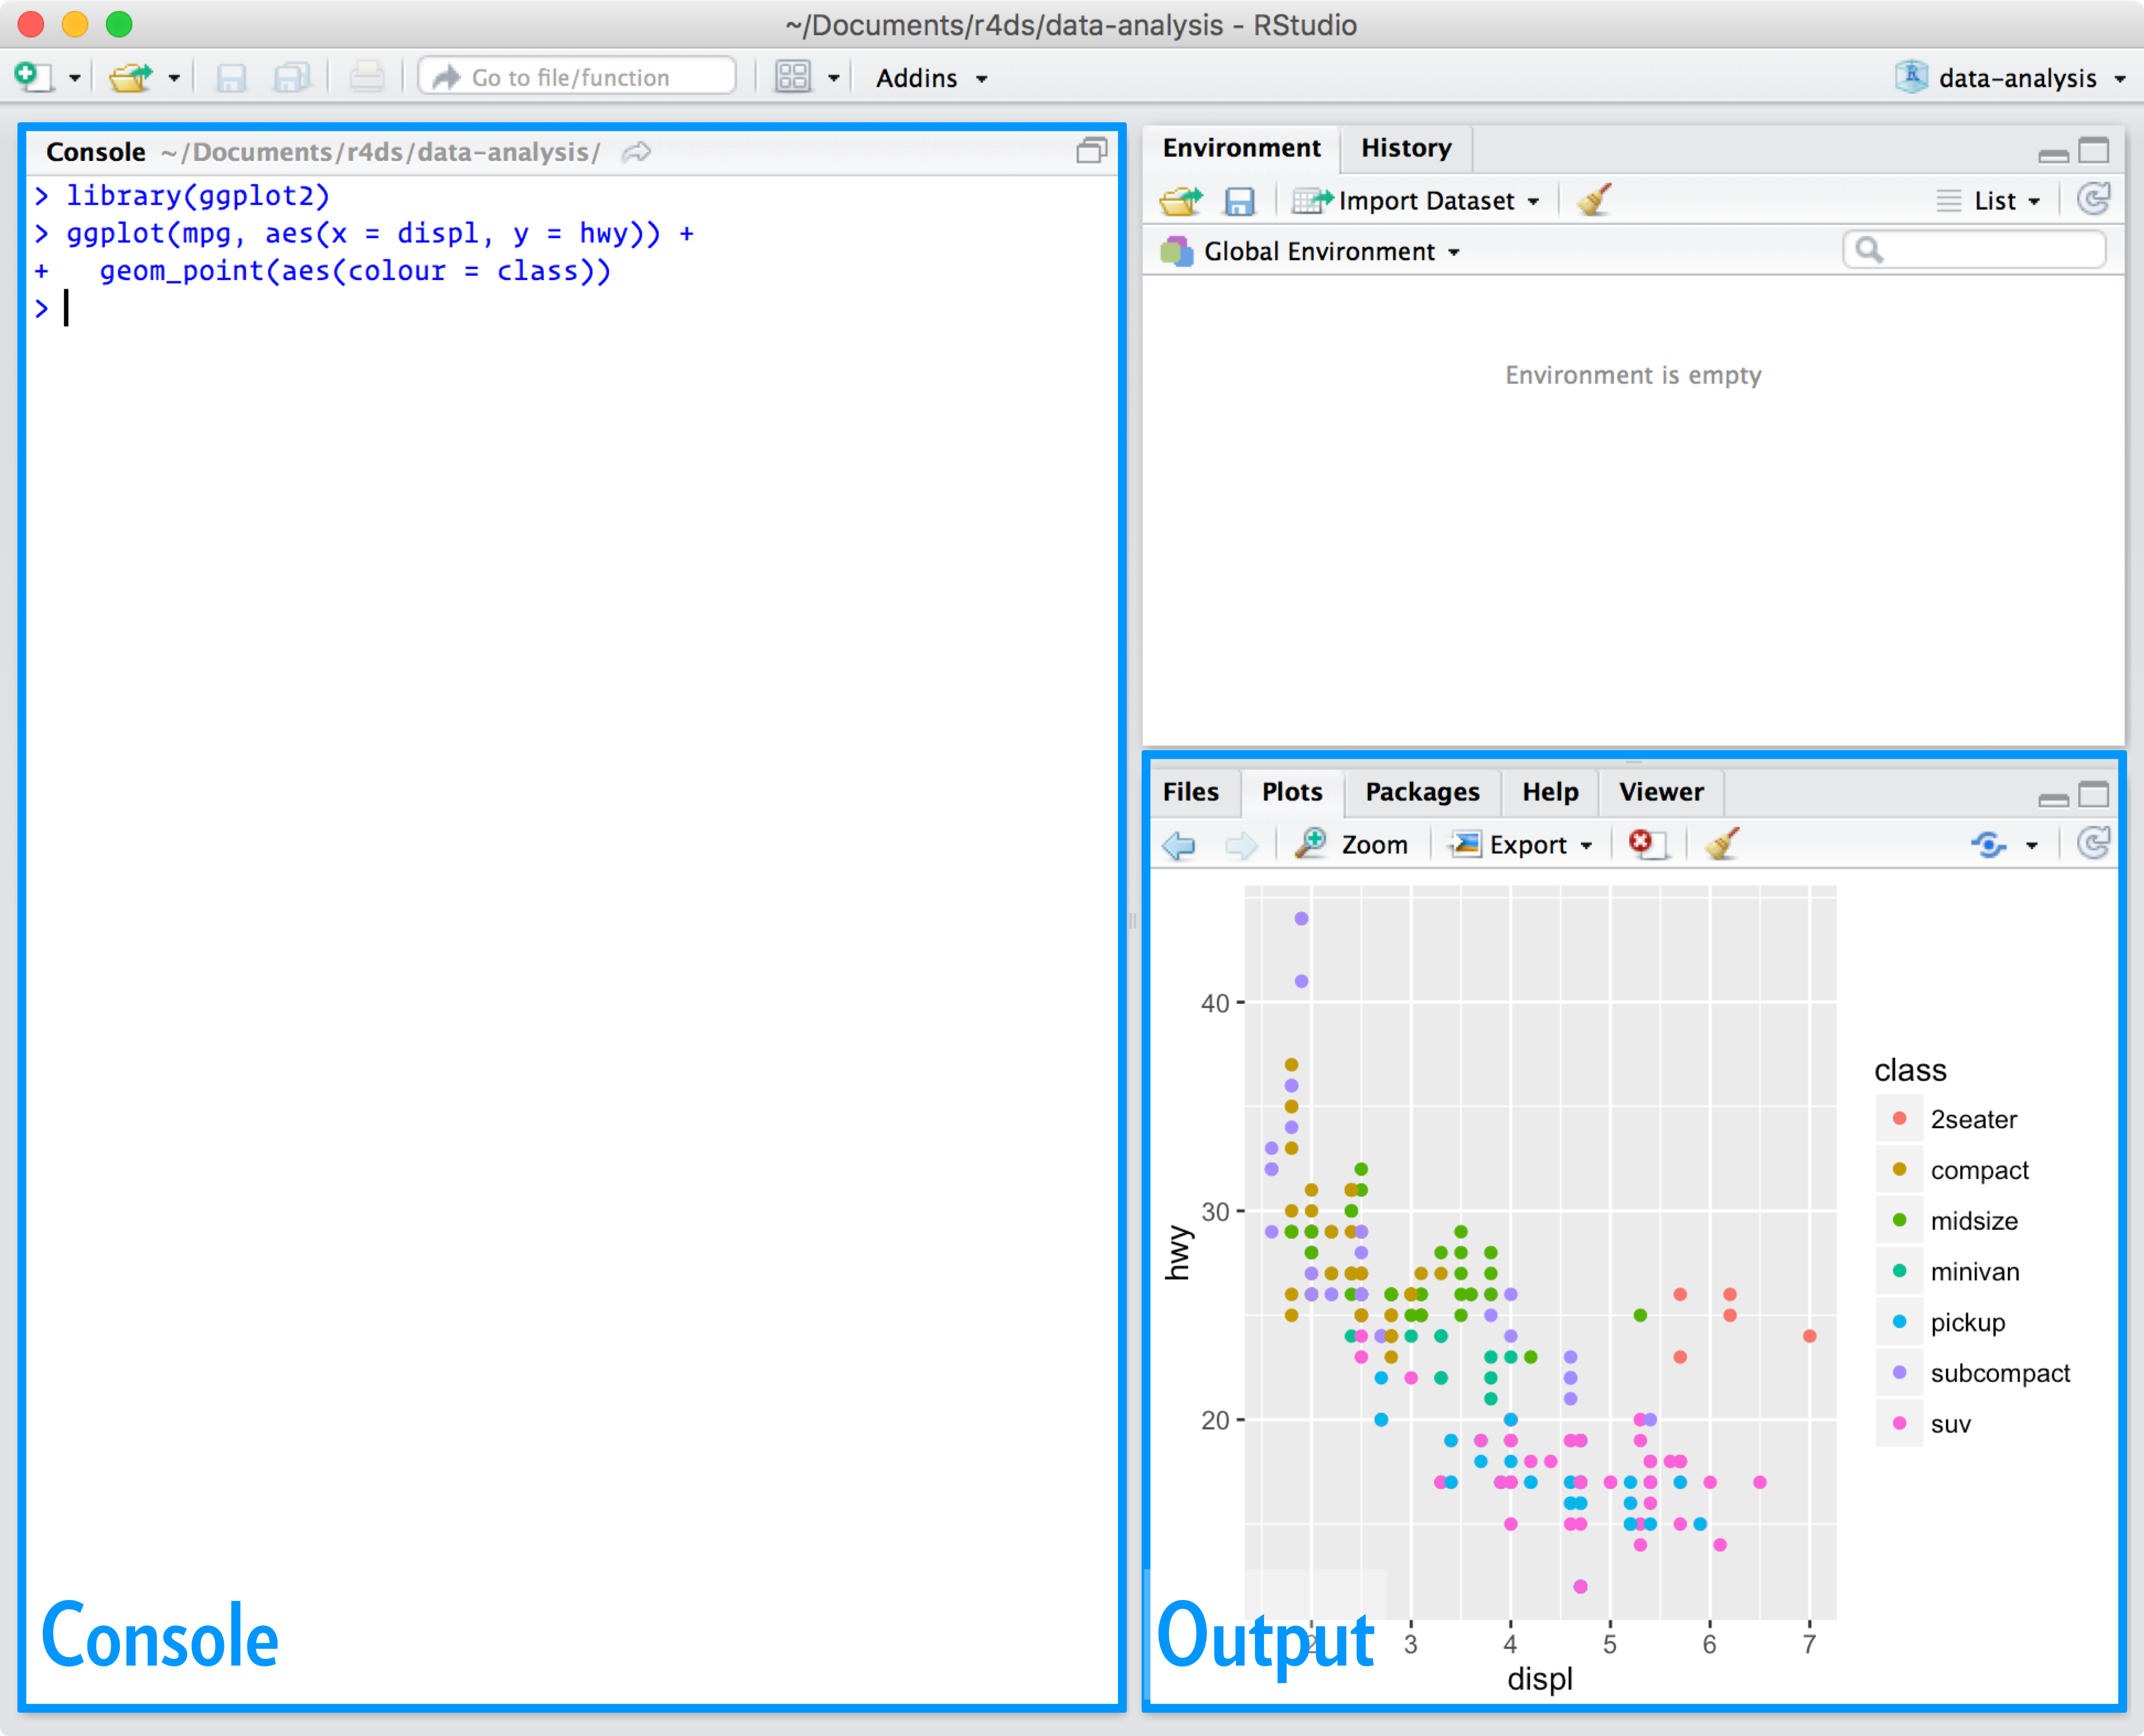
\includegraphics[width=0.9\linewidth]{imagens/rstudio-console} \end{center}

Do lado esquerdo fica o console, onde os comandos podem ser digitados e onde ficam os \emph{outputs}.

No lado superior direito há duas abas:

-i) \emph{Environment}, que é onde ficam armazendos os objetos criados, bases de dados importadas, etc; e

-ii) \emph{History}, onde ficam o histórico dos comandos executados.

A forma mais eficiente e prática de usar o R ou o RStudio é através de um \emph{script}. No RStudio, vá em \emph{File} → \emph{New File} → \emph{R Script}. A interface agora fica dividida em 4 partes:

\begin{center}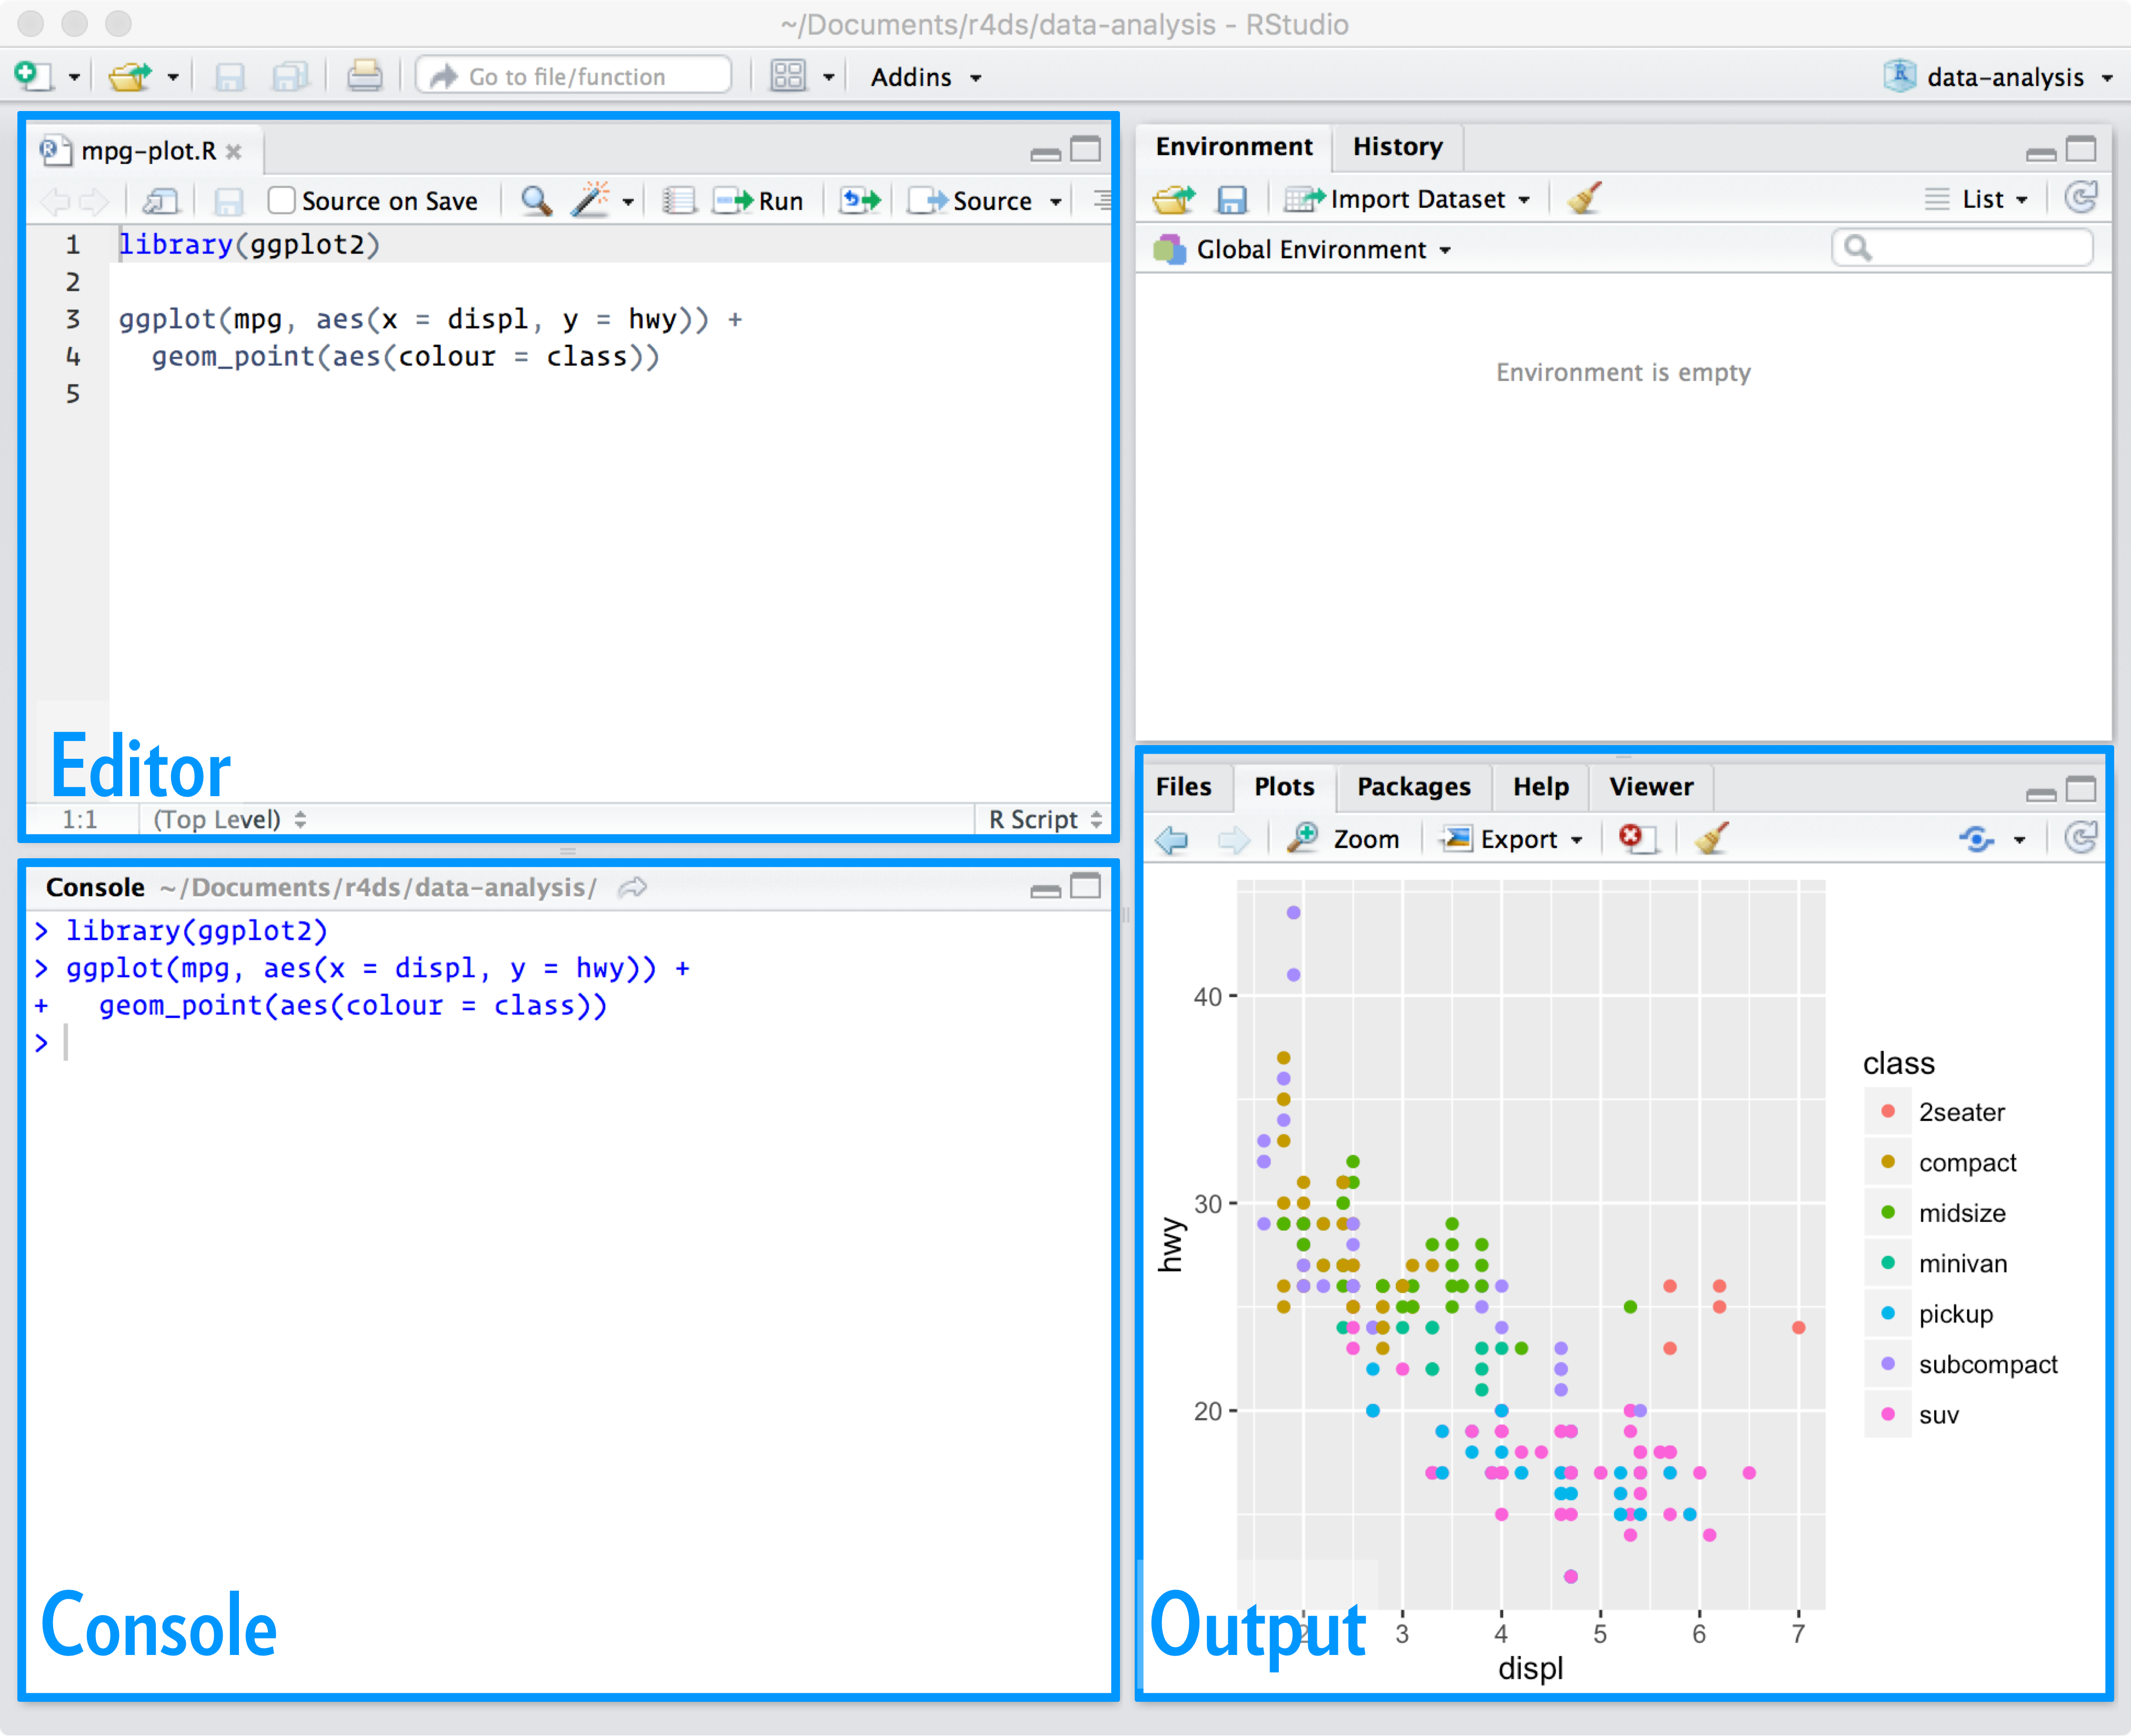
\includegraphics[width=0.9\linewidth]{imagens/rstudio-editor} \end{center}

No \emph{script} você pode digitar comandos a serem executados e também comentários.

\hypertarget{objetos-r}{%
\section{Objetos R}\label{objetos-r}}

R possui cinco classes básicas ou ``atômicas'' de objetos:

\begin{itemize}
\item
  character
\item
  numeric (real numbers)
\item
  integer
\item
  complex
\item
  logical (True/False)
\end{itemize}

O tipo mais básico de objeto R é um vetor. Vetores vazios podem ser criados com a função \texttt{vector()}. Existe apenas uma regra sobre vetores em R, que um vetor pode conter apenas objetos da mesma classe.

Mas há uma exceção, que é uma lista. Uma lista é representada como um vetor, mas pode conter objetos de diferentes classes. De fato, geralmente é por isso que os usamos.

\hypertarget{swirl}{%
\section{\texorpdfstring{\emph{swirl}}{swirl}}\label{swirl}}

O \emph{swirl} é um pacote do R construído para transformar o console em uma ferramenta interativa para aprender R. \emph{swirl} ensina programação de R e ciência de dados interativamente, no seu próprio ritmo e diretamente no console do R. Para entender melhor o projeto, veja \url{http://swirlstats.com/} e \url{http://swirlstats.com/students}. Nestes endereços são dados os detalhes sobre como usar o \emph{swirl}. Uma vez intalado e carregado o pacote, você é levado a efetuar tarefas:

\begin{center}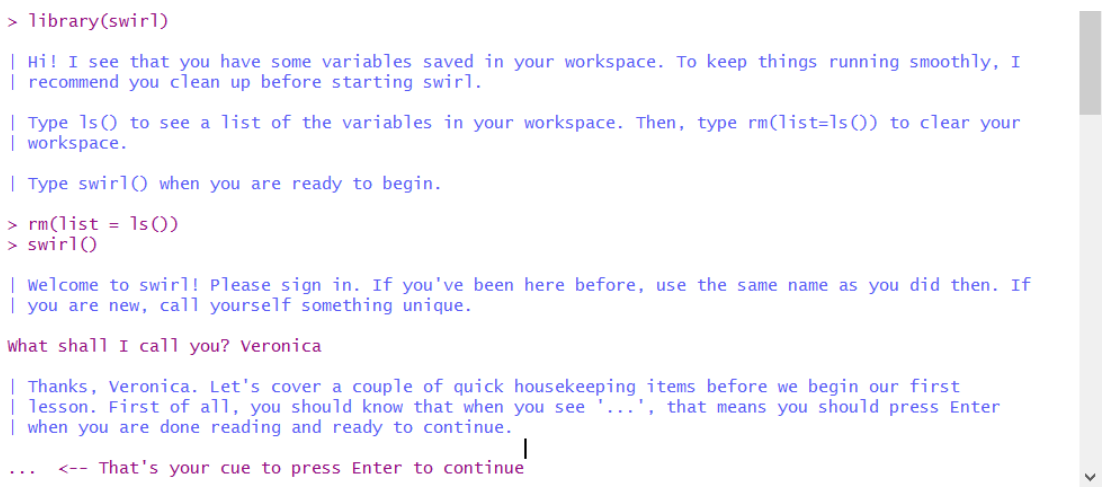
\includegraphics[width=0.9\linewidth]{imagens/swirl} \end{center}

O \emph{swirl} dá acesso às tarefas de cursos de R que estão disponíveis também no Coursera, como o \emph{R Programming}: \emph{The basics of programming in R}, em \url{https://pt.coursera.org/learn/r-programming}. Além deste, estão
disponíveis no \emph{swirl}: \emph{Regression Models: The basics of regression modeling in R, Statistical Inference: The basics of statistical inference in R, e Exploratory Data Analysis: The basics of exploring data in R}.

\hypertarget{literature}{%
\chapter{Tibbles x Data frames}\label{literature}}

\begin{quote}
``Famílias felizes são todas iguais; toda família infeliz é infeliz à sua maneira.'' -- Leo Tolstoi
\end{quote}

O que é um \emph{tibble}? \emph{Tibbles} são similares aos \emph{data frames}, porém diferentes em dois aspectos: \textbf{impressão} e \textbf{indexação}

Na impressão no console, os \emph{tibbles} apresentam apenas as dez primeiras linhas e todas as colunas que cabem na tela, tornando mais fácil o trabalho com grandes volumes de dados. Além disso, cada coluna apresenta o seu tipo, algo semelhante ao apresentado quando utilizamos a função \texttt{str()}. A segunda diferença, não menos importante, é a forma de indexação. Para indexar um \texttt{tibble} devemos utilizar o nome completo da variável que desejamos. Caso contrário, ocorrerá um erro.

Ainda sobre a indexação, sempre que indexarmos um \texttt{tibble} usando \texttt{{[}}, o resultado será outro \texttt{tibble}. Usando \texttt{{[}{[}} o resultados será um vetor.

Em síntese, \emph{data frames} são tabelas de dados. Em seu formato, são bem parecidos com as matrizes, no entanto, possuem algumas diferenças significativas. Podemos idealizar os \emph{data frames} como sendo matrizes em que cada coluna pode armazenar um tipo de dado diferente. Logo, estamos lidando com um objeto bem mais versátil do que as matrizes e os vetores.

Uma das funções básicas mais importantes para começarmos a trabalhar com \emph{data frames} é a \texttt{str()}. Essa função dá uma visão clara da estrutura do nosso objeto, bem como informa os tipos de dados existentes.

A função \texttt{View()} chama um visualizador de dados no estilo de planilhas em um objeto R. Semelhante a planilha do excel.

\begin{Shaded}
\begin{Highlighting}[]
\KeywordTok{View}\NormalTok{(x, title)}
\end{Highlighting}
\end{Shaded}

Os argumentos da função são: \texttt{x} um objeto do R que pode ser coagido a um quadro de dados. E \texttt{title}, título para a janela do visualizador. O padrão é o nome de x prefixado.

\hypertarget{o-que-uxe9-dados-organizados}{%
\section{O que é Dados organizados?}\label{o-que-uxe9-dados-organizados}}

\begin{quote}
``Os conjuntos de dados organizados são todos iguais, mas todos os conjuntos de dados confusos são confusos à sua maneira.'' -- Hadley Wickham
\end{quote}

Costuma-se dizer que 80\% da análise de dados é gasta no processo de limpeza e preparação os dados (Dasu e Johnson 2003). A preparação de dados não é apenas um primeiro passo, mas deve ser repetidos muitos ao longo da análise, à medida que novos problemas surgem ou novos dados são coletados.Você vai precisar instalar os pacotes \texttt{tidyr}, \texttt{devtools} e \texttt{DSR}. Para instalar \texttt{tidyr} e \texttt{devtools}, abra o RStudio e execute o comando:

\begin{Shaded}
\begin{Highlighting}[]
\KeywordTok{install.packages}\NormalTok{(}\KeywordTok{c}\NormalTok{(}\StringTok{"tidyr"}\NormalTok{, }\StringTok{"devtools"}\NormalTok{))}
\end{Highlighting}
\end{Shaded}

\texttt{DSR} é uma coleção de conjuntos de dados. Para instalar DSR, execute o comando:

\begin{Shaded}
\begin{Highlighting}[]
\NormalTok{devtools}\OperatorTok{::}\KeywordTok{install_github}\NormalTok{(}\StringTok{"garrettgman/DSR"}\NormalTok{)}
\end{Highlighting}
\end{Shaded}

Os dados tabulares podem ser organizados de várias maneiras. Os conjuntos de dados abaixo mostram os mesmos dados organizados de quatro maneiras diferentes, sendo que possuem as mesmas variáveis: país, ano, população e casos. Mas cada conjunto organiza os valores em forma de layout diferente. Vejamos essas tabelas de dados seguintes:

\begin{Shaded}
\begin{Highlighting}[]
\KeywordTok{library}\NormalTok{(DSR)}
\CommentTok{# Primeiro conjunto de dados.}
\NormalTok{table1}
\end{Highlighting}
\end{Shaded}

\begin{verbatim}
## # A tibble: 6 x 4
##   country      year  cases population
##   <fct>       <int>  <int>      <int>
## 1 Afghanistan  1999    745   19987071
## 2 Afghanistan  2000   2666   20595360
## 3 Brazil       1999  37737  172006362
## 4 Brazil       2000  80488  174504898
## 5 China        1999 212258 1272915272
## 6 China        2000 213766 1280428583
\end{verbatim}

\begin{Shaded}
\begin{Highlighting}[]
\CommentTok{# Segundo conjunto de dados.}
\NormalTok{table2}
\end{Highlighting}
\end{Shaded}

\begin{verbatim}
## # A tibble: 12 x 4
##    country      year key             value
##    <fct>       <int> <fct>           <int>
##  1 Afghanistan  1999 cases             745
##  2 Afghanistan  1999 population   19987071
##  3 Afghanistan  2000 cases            2666
##  4 Afghanistan  2000 population   20595360
##  5 Brazil       1999 cases           37737
##  6 Brazil       1999 population  172006362
##  7 Brazil       2000 cases           80488
##  8 Brazil       2000 population  174504898
##  9 China        1999 cases          212258
## 10 China        1999 population 1272915272
## 11 China        2000 cases          213766
## 12 China        2000 population 1280428583
\end{verbatim}

\begin{Shaded}
\begin{Highlighting}[]
\CommentTok{# Terceiro conjunto de dados.}
\NormalTok{table3}
\end{Highlighting}
\end{Shaded}

\begin{verbatim}
## # A tibble: 6 x 3
##   country      year rate             
##   <fct>       <int> <chr>            
## 1 Afghanistan  1999 745/19987071     
## 2 Afghanistan  2000 2666/20595360    
## 3 Brazil       1999 37737/172006362  
## 4 Brazil       2000 80488/174504898  
## 5 China        1999 212258/1272915272
## 6 China        2000 213766/1280428583
\end{verbatim}

O último conjunto de dados é uma coleção de duas tabelas.

\begin{Shaded}
\begin{Highlighting}[]
\CommentTok{# Quarto conjunto de dados.}
\NormalTok{table4 }\CommentTok{# cases}
\end{Highlighting}
\end{Shaded}

\begin{verbatim}
## # A tibble: 3 x 3
##   country     `1999` `2000`
##   <fct>        <int>  <int>
## 1 Afghanistan    745   2666
## 2 Brazil       37737  80488
## 3 China       212258 213766
\end{verbatim}

\begin{Shaded}
\begin{Highlighting}[]
\NormalTok{table5 }\CommentTok{# population}
\end{Highlighting}
\end{Shaded}

\begin{verbatim}
## # A tibble: 3 x 3
##   country         `1999`     `2000`
##   <fct>            <int>      <int>
## 1 Afghanistan   19987071   20595360
## 2 Brazil       172006362  174504898
## 3 China       1272915272 1280428583
\end{verbatim}

R segue um conjunto de convenções que tornam um layout de dados tabulares muito mais fácil de trabalhar do que outros. Seus dados serão mais fáceis de trabalhar no R se seguirem três regras:

\begin{itemize}
\tightlist
\item
  1.Cada variável no conjunto de dados é colocada em sua própria coluna;
\item
  2.Cada observação é colocada em sua própria linha;
\item
  3.Cada valor é colocado em sua própria célula.
\end{itemize}

Os dados que satisfazem essas regras são conhecidos como dados organizados. Observe que \texttt{table1} são dados organizados.

\begin{center}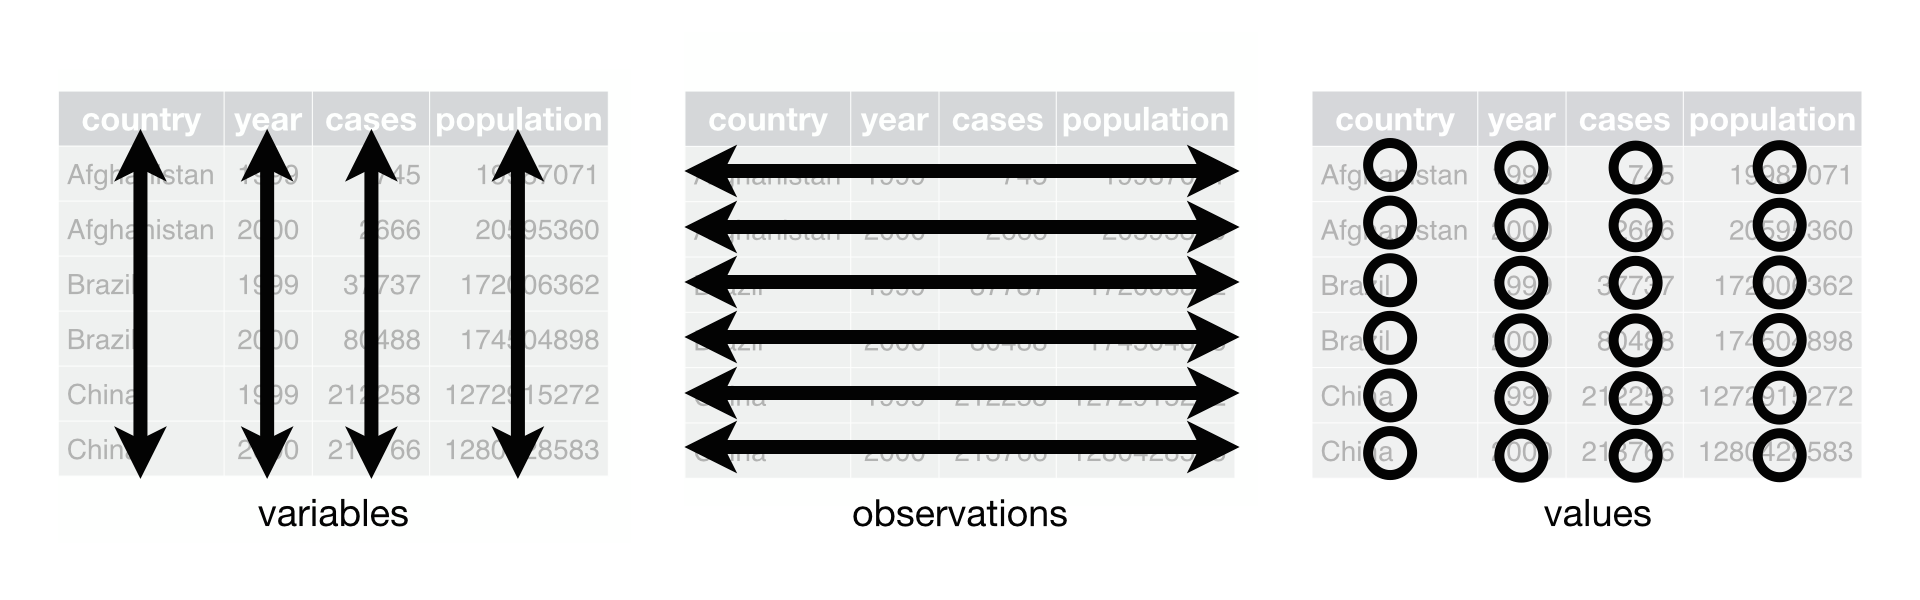
\includegraphics[width=0.9\linewidth]{imagens/tidy-1} \end{center}

Em \texttt{table1}, cada variável é colocada em sua própria coluna, cada observação em sua própria linha e cada valor em sua própria célula.

\hypertarget{operador-pipe}{%
\section{\texorpdfstring{Operador \emph{pipe} \texttt{\%\textgreater{}\%}}{Operador pipe \%\textgreater\%}}\label{operador-pipe}}

\begin{center}
\includegraphics[width=0.25\linewidth]{imagens/magritt} \end{center}

O pacote \texttt{magrittr} oferece um conjunto de operadores que promovem semânticas que melhorara seu código que deixa mais claro a compreensão:

\begin{itemize}
\tightlist
\item
  estruturar seqüências de operações de dados da esquerda para a direita (em oposição a de dentro e de fora);
\item
  evitando chamadas de função aninhadas;
\item
  minimizar a necessidade de variáveis locais e definições de função, e
  facilitando a adição de etapas em qualquer lugar da sequência de operações.
\end{itemize}

\hypertarget{recursos}{%
\subsection{Recursos}\label{recursos}}

Tubulação básica:

\begin{itemize}
\tightlist
\item
  x \texttt{\%\textgreater{}\%} \textbf{f} é equivalente a \textbf{f(x)};
\item
  x \texttt{\%\textgreater{}\%} \textbf{f(y)} é equivalente a \textbf{f(x, y)};
\item
  x \texttt{\%\textgreater{}\%} \textbf{f} \texttt{\%\textgreater{}\%} \textbf{g} \texttt{\%\textgreater{}\%} \textbf{h} é equivalente a \textbf{h(g(f(x)))}.
\end{itemize}

O operador do \textbf{pipeline} \texttt{\%\textgreater{}\%} é muito útil para reunir várias funções em uma sequência de operações. Os tubos são uma ferramenta poderosa para expressar claramente as operações. O \textbf{pipe}, \texttt{\%\textgreater{}\%} vem do pacote \texttt{magrittr} de Stefan Milton Bache. Pacotes no \texttt{tidyverse} carregam \texttt{\%\textgreater{}\%} automaticamente, para que normalmente não carregue o magrittr explicitamente.

\begin{quote}
third(second(first(x)))
\end{quote}

Para começar a utilizar o \emph{pipe}, instale e carregue o pacote \texttt{magrittr}.

\begin{Shaded}
\begin{Highlighting}[]
\KeywordTok{install.packages}\NormalTok{(}\StringTok{"magrittr"}\NormalTok{)}
\KeywordTok{library}\NormalTok{(magrittr)}
\end{Highlighting}
\end{Shaded}

Para mais informações sobre o \emph{pipe}, outros operadores relacionados e exemplos de utilização, visite a página \href{https://cran.r-project.org/web/packages/magrittr/vignettes/magrittr.html}{Ceci n'est pas un pipe}. Ou consulte a vinheta do pacote \texttt{vignette("magrittr")}.

\hypertarget{breve-introduuxe7uxe3o-ao-tidyr}{%
\section{\texorpdfstring{Breve Introdução ao \texttt{tidyr}}{Breve Introdução ao tidyr}}\label{breve-introduuxe7uxe3o-ao-tidyr}}

\begin{center}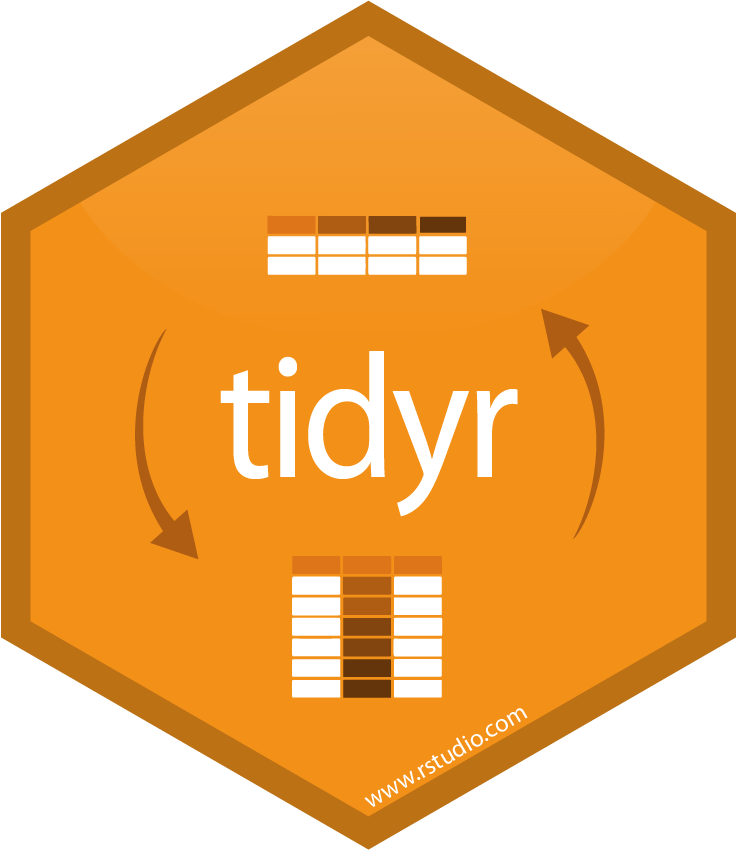
\includegraphics[width=0.25\linewidth]{imagens/tidyr} \end{center}

O pacote tidyr tem como principal objetivo transformar um data frame para o formato tidy, ou limpo.

De acordo com as regras ditas anteriormente, um dado limpo/organizado é aquele com formato \emph{long}, ou seja, com mais linhas. O outro formato é chamado de \emph{wide}, com mais colunas. No caso deste exemplo, ano é uma variável, logo é necessário existir uma coluna com os valores de ano. O valor relacionado a UF naqueles anos também é outra variável, então precisa de uma coluna pra representá-lo. Além disso, a própria UF precisa de uma coluna.

O \texttt{tidyr} possui duas funções principais:

\texttt{gather}: Transforma um \texttt{tibble} \emph{wide} em \emph{long}, ou seja, transforma os dados no formato \emph{tidy}.

\texttt{spread}: Transforma um \texttt{tibble} \emph{long} em \emph{wide}, ou seja, transforma dados que estão no formato \emph{tidy} em formato não \emph{tidy}.

Além disso, existem duas funções que podem ser importantes na nossa análise: \texttt{separate} e \texttt{unite}, que separa uma coluna em duas e vice versa.

\hypertarget{gather}{%
\subsection{\texorpdfstring{\texttt{gather()}}{gather()}}\label{gather}}

Vamos criar um \texttt{tibble} no formato \emph{wide} e transformá-lo em um dado \emph{tidy}:

\begin{Shaded}
\begin{Highlighting}[]
\KeywordTok{library}\NormalTok{(tibble)}
\NormalTok{dados_wide <-}\StringTok{ }\KeywordTok{tibble}\NormalTok{(}\DataTypeTok{uf =} \KeywordTok{c}\NormalTok{(}\StringTok{"RJ"}\NormalTok{, }\StringTok{"SP"}\NormalTok{), }\StringTok{`}\DataTypeTok{2017}\StringTok{`}\NormalTok{ =}\StringTok{ }\KeywordTok{c}\NormalTok{(}\DecValTok{10}\NormalTok{, }\DecValTok{11}\NormalTok{), }\StringTok{`}\DataTypeTok{2018}\StringTok{`}\NormalTok{ =}\StringTok{ }\KeywordTok{c}\NormalTok{(}\DecValTok{11}\NormalTok{, }\DecValTok{10}\NormalTok{))}
\NormalTok{dados_wide}
\end{Highlighting}
\end{Shaded}

\begin{verbatim}
## # A tibble: 2 x 3
##   uf    `2017` `2018`
##   <chr>  <dbl>  <dbl>
## 1 RJ        10     11
## 2 SP        11     10
\end{verbatim}

a função \texttt{gather()} retorna um \texttt{tibble} com duas colunas, por padrão, isso se não inserirmos nenhum parâmetro além do \texttt{tibble}.

\hypertarget{exercuxedcios}{%
\subsection{Exercícios}\label{exercuxedcios}}

\begin{itemize}
\tightlist
\item
  1.Qual a diferença entre uma matriz e um data frame no R?
\item
  2.Os data frames podem ser indexados com a mesma sintaxe utilizada para matrizes?
\item
  3.Qual função básica que utilizamos para verificar a estrutura dos dados de um data frame?
\end{itemize}

\hypertarget{exercuxedcios-1}{%
\subsection{Exercícios}\label{exercuxedcios-1}}

\begin{itemize}
\item
  \begin{enumerate}
  \def\labelenumi{\arabic{enumi}.}
  \tightlist
  \item
    Reescreva a expressão abaixo utilizando o \texttt{\%\textgreater{}\%}.
  \end{enumerate}
\end{itemize}

\begin{quote}
round(mean(sum(1:10)/3), digits = 1)
\end{quote}

\textbf{Dica}: utilize a função \texttt{magrittr::divide\_by()}. Veja o help da função para mais informações.

\begin{itemize}
\item
  \begin{enumerate}
  \def\labelenumi{\arabic{enumi}.}
  \setcounter{enumi}{1}
  \tightlist
  \item
    Reescreva o código abaixo utilizando o \texttt{\%\textgreater{}\%}.
  \end{enumerate}
\end{itemize}

\begin{quote}
x \textless- rnorm(100)
x.pos \textless- x{[}x\textgreater0{]}
media \textless- mean(x.pos)
saida \textless- round(media, 1)
\end{quote}

\begin{itemize}
\item
  \begin{enumerate}
  \def\labelenumi{\arabic{enumi}.}
  \setcounter{enumi}{2}
  \tightlist
  \item
    Sem rodar, diga qual a saída do código abaixo. Consulte o \texttt{help} das funções caso precise.
  \end{enumerate}
\end{itemize}

\begin{quote}
2 \%\textgreater\%
add(2) \%\textgreater\%
c(6, NA) \%\textgreater\%
mean(na.rm = T) \%\textgreater\%
equals(5)
\end{quote}

\hypertarget{method}{%
\chapter{\texorpdfstring{Manipulando Data Frames com \texttt{dplyr}}{Manipulando Data Frames com dplyr}}\label{method}}

Entendamos a manipulação de dados como o ato de transformar, reestruturar, limpar, agregar e juntar os dados. Para se ter uma noção da importância dessa fase, alguns estudiosos da área de Ciência de Dados costumam afirmar que 80\% do trabalho é encontrar uma boa fonte de dados, limpar e preparar os dados, sendo que os 20\% restantes seriam o trabalho de aplicar modelos e realizar alguma análise propriamente dita.

\hypertarget{o-pacote-dplyr}{%
\section{\texorpdfstring{O Pacote \texttt{dplyr}}{O Pacote dplyr}}\label{o-pacote-dplyr}}

O pacote \texttt{dplyr} foi desenvolvido por Hadley Wickham, cientista chefe do RStudio. É uma versão otimizada do pacote \texttt{plyr}. O pacote \texttt{dplyr} não fornece nenhuma funcionalidade ``nova'' ao R, pois já é feito com base no R, mas simplifica \textbf{bastante} a funcionalidade no R.

Uma contribuição importante do \texttt{dplyr} é que ele fornece uma ``gramática'' (em particular, verbos) para manipulação

\hypertarget{gramuxe1tica-do-dplyr}{%
\section{\texorpdfstring{Gramática do \texttt{dplyr}}{Gramática do dplyr}}\label{gramuxe1tica-do-dplyr}}

Alguns dos principais ``verbos'' básicos de tablea única fornecidos pelo \texttt{dplyr} são:

-\texttt{select}: retorna um subconjunto das colunas de um data.frames, usando uma notação flexível;

\begin{itemize}
\tightlist
\item
  \texttt{pull()}: retire uma única variável;
\end{itemize}

-\texttt{filter}: extrair um subconjunto de linhas(observações) de um data.frames com base em condições lógicas;

-\texttt{arrange}: reordenar linhas de um data.frames;

-\texttt{rename}: renomear variáveis em um data.frames;

-\texttt{mutate}: adiciona novas variáveis/colunas ou transforme variáveis existentes;

-\texttt{summarise/summarize}: gera estatísticas resumidas de diferentes variáveis no data.frames, possivelmente dentro dos estratos.

\hypertarget{propriedades-das-funuxe7uxf5es-do-dplyr}{%
\section{\texorpdfstring{Propriedades das funções do \texttt{dplyr}}{Propriedades das funções do dplyr}}\label{propriedades-das-funuxe7uxf5es-do-dplyr}}

As funções têm algumas características comuns:

-1.O primeiro argumento é um data.frames;

-2.Os argumentos subsequentes descrevem o que fazer com o data.frames especificado no primeiro argumento;

-3.O resultado de retorno de uma função é um novo data.frames;

-4.Os data.frames devem devidamente formatados e anotados para que tudo isso seja útil. Em particular, os dados devem estar \emph{organizados}.

\hypertarget{instalando-o-pacote-dplyr}{%
\section{\texorpdfstring{Instalando o Pacote \texttt{dplyr}}{Instalando o Pacote dplyr}}\label{instalando-o-pacote-dplyr}}

O pacote pode ser instalado a partir do CRAN ou do GitHub usando o pacote \texttt{devtools} com a função \texttt{install\_github()}. O repositório GitHub normalmente contém as versões mais atualizadas dos pacotes.

Para instalar a partir do CRAN, bastar executar:

\begin{Shaded}
\begin{Highlighting}[]
\KeywordTok{install.packages}\NormalTok{(}\StringTok{"dplyr"}\NormalTok{)}
\end{Highlighting}
\end{Shaded}

Para instalar a partir do GitHub, execute:

\begin{Shaded}
\begin{Highlighting}[]
\KeywordTok{library}\NormalTok{(devtools) }\CommentTok{#carregar o pacote 'devtools' antes.}
\NormalTok{devtools}\OperatorTok{::}\KeywordTok{install_github}\NormalTok{(}\StringTok{"hadley/dplyr"}\NormalTok{)}
\end{Highlighting}
\end{Shaded}

Após a instalação do pacote, carregá-lo com a função \texttt{library()}:

\begin{Shaded}
\begin{Highlighting}[]
\KeywordTok{library}\NormalTok{(dplyr)}
\end{Highlighting}
\end{Shaded}

Ao carregar o pacote você pode receber alguns avisos, porque há funções no \texttt{dplyr}que têm o mesmo nome que as funções em outros pacotes. Por enquanto pode ignorar os avisos.

\hypertarget{select}{%
\section{\texorpdfstring{\texttt{select()}}{select()}}\label{select}}

Para melhor apresentar as funcionalidades da função, usaremos um conjunto de dados diários sobre poluição do ar e taxa de mortalidade da \href{http://www.biostat.jhsph.edu/~rpeng/leanpub/rprog/chicago_data.zip}{cidade de Chicago}, nos EUA.

Você pode carregar os dados no R usando a função \texttt{readRDS()}:

\begin{Shaded}
\begin{Highlighting}[]
\NormalTok{chicago <-}\StringTok{ }\KeywordTok{readRDS}\NormalTok{(}\StringTok{"data/chicago.rds"}\NormalTok{)}
\end{Highlighting}
\end{Shaded}

Este banco de dados encontra no seguinte endereço: \url{http://www.biostat.jhsph.edu/~rpeng/leanpub/rprog/chicago_data.zip} e está em um arquivo zipado. Uma das formas para facilitar o processo de descompactação do arquivo pelo R é:

\begin{Shaded}
\begin{Highlighting}[]
\CommentTok{# objeto caracter, endereço do arquivo.}
\NormalTok{fileURL <-}\StringTok{ "http://www.biostat.jhsph.edu/~rpeng/leanpub/rprog/chicago_data.zip"}

\CommentTok{#Esta função pode ser usada para baixar um arquivo da Internet.}
\KeywordTok{download.file}\NormalTok{(fileURL, }\DataTypeTok{destfile =} \StringTok{"data/chicago.rds"}\NormalTok{, }\DataTypeTok{method =} \StringTok{"curl"}\NormalTok{, }\DataTypeTok{extra=}\StringTok{'-L'}\NormalTok{) }
\end{Highlighting}
\end{Shaded}

Descrição do banco: tem 8 colunas e 6940 linhas. Cada linha refere-se a um dia. As colunas são:

\begin{itemize}
\tightlist
\item
  city:

  \begin{itemize}
  \tightlist
  \item
    cidade, neste campo tem apenas ``chic'' referenciando a cidade de Chicago.
  \end{itemize}
\item
  tmpd:

  \begin{itemize}
  \tightlist
  \item
    temperatura em Fahrenheit.
  \end{itemize}
\item
  dptp:

  \begin{itemize}
  \tightlist
  \item
    temperatura do ponto de orvalho.
  \end{itemize}
\item
  date:

  \begin{itemize}
  \tightlist
  \item
    tempo em dias.
  \end{itemize}
\item
  pm25tmean2:

  \begin{itemize}
  \tightlist
  \item
    partículas médias \textless{} 2,5mg por m cúbico (mais perigoso).
  \end{itemize}
\item
  pm10tmean2:

  \begin{itemize}
  \tightlist
  \item
    partículas médias em 2,5\^{}-10 por m cúbico.
  \end{itemize}
\item
  o3tmean2:

  \begin{itemize}
  \tightlist
  \item
    Ozônio em partes por bilhão.
  \end{itemize}
\item
  no2tmean2:

  \begin{itemize}
  \tightlist
  \item
    Medição mediana de dióxido de sulfato.
  \end{itemize}
\end{itemize}

Umas das formas de ter informações do seu banco de dados é utilizar as seguintes funções \texttt{dim()} e \texttt{str()}. A primeira especifica a dimensão do seu banco e a segunda a estrutura do seu banco de dados.

\begin{Shaded}
\begin{Highlighting}[]
\KeywordTok{dim}\NormalTok{(chicago)}
\end{Highlighting}
\end{Shaded}

\begin{verbatim}
## [1] 6940    8
\end{verbatim}

\begin{Shaded}
\begin{Highlighting}[]
\KeywordTok{str}\NormalTok{(chicago)}
\end{Highlighting}
\end{Shaded}

\begin{verbatim}
## 'data.frame':    6940 obs. of  8 variables:
##  $ city      : chr  "chic" "chic" "chic" "chic" ...
##  $ tmpd      : num  31.5 33 33 29 32 40 34.5 29 26.5 32.5 ...
##  $ dptp      : num  31.5 29.9 27.4 28.6 28.9 ...
##  $ date      : Date, format: "1987-01-01" "1987-01-02" ...
##  $ pm25tmean2: num  NA NA NA NA NA NA NA NA NA NA ...
##  $ pm10tmean2: num  34 NA 34.2 47 NA ...
##  $ o3tmean2  : num  4.25 3.3 3.33 4.38 4.75 ...
##  $ no2tmean2 : num  20 23.2 23.8 30.4 30.3 ...
\end{verbatim}

Muitas vezes teremos um data.frames contendo um grande número de dados. Com isso, a função \texttt{select()} permite obter as poucas colunas que você pode precisar.

Suponhamos que desejássemos pegar as 3 primeiras colunas. Há algumas maneiras de fazer isto. Poderíamos, por exemplo, usar o índices númericos. Mas também podemos usar os nomes diretamente.

\begin{Shaded}
\begin{Highlighting}[]
\KeywordTok{names}\NormalTok{(chicago[}\DecValTok{1}\OperatorTok{:}\DecValTok{3}\NormalTok{]) }
\end{Highlighting}
\end{Shaded}

\begin{verbatim}
## [1] "city" "tmpd" "dptp"
\end{verbatim}

\begin{Shaded}
\begin{Highlighting}[]
\NormalTok{subset1 <-}\StringTok{ }\KeywordTok{select}\NormalTok{(chicago, city}\OperatorTok{:}\NormalTok{dptp)}
\KeywordTok{head}\NormalTok{(subset1)}
\end{Highlighting}
\end{Shaded}

\begin{verbatim}
##   city tmpd   dptp
## 1 chic 31.5 31.500
## 2 chic 33.0 29.875
## 3 chic 33.0 27.375
## 4 chic 29.0 28.625
## 5 chic 32.0 28.875
## 6 chic 40.0 35.125
\end{verbatim}

Normalmente \texttt{:} não pode ser usado com nomes ou sequências de caracteres, mas dentro da função \texttt{select()} pode usá-lo para especificar um intervalo de nomes de variáveis.

Pode \textbf{omitir} variáveis usando a função \texttt{select()} usando o sinal negativo.

\begin{Shaded}
\begin{Highlighting}[]
\NormalTok{subset2 <-}\StringTok{ }\KeywordTok{select}\NormalTok{(chicago, }\OperatorTok{-}\NormalTok{(city}\OperatorTok{:}\NormalTok{dptp))}
\KeywordTok{head}\NormalTok{(subset2)}
\end{Highlighting}
\end{Shaded}

\begin{verbatim}
##         date pm25tmean2 pm10tmean2 o3tmean2 no2tmean2
## 1 1987-01-01         NA   34.00000 4.250000  19.98810
## 2 1987-01-02         NA         NA 3.304348  23.19099
## 3 1987-01-03         NA   34.16667 3.333333  23.81548
## 4 1987-01-04         NA   47.00000 4.375000  30.43452
## 5 1987-01-05         NA         NA 4.750000  30.33333
## 6 1987-01-06         NA   48.00000 5.833333  25.77233
\end{verbatim}

o que indica que estamos incluindo todas as variáveis, exceto as variáveis \texttt{city} até \texttt{dptp}.

O código equivalente ao anterior sem o uso do pacote seria:

\begin{Shaded}
\begin{Highlighting}[]
\NormalTok{i <-}\StringTok{ }\KeywordTok{match}\NormalTok{(}\StringTok{"city"}\NormalTok{, }\KeywordTok{names}\NormalTok{(chicago))}
\NormalTok{j <-}\StringTok{ }\KeywordTok{match}\NormalTok{(}\StringTok{"dptp"}\NormalTok{, }\KeywordTok{names}\NormalTok{(chicago))}
\KeywordTok{head}\NormalTok{(chicago[, }\OperatorTok{-}\NormalTok{(i}\OperatorTok{:}\NormalTok{j)])}
\end{Highlighting}
\end{Shaded}

\begin{verbatim}
##         date pm25tmean2 pm10tmean2 o3tmean2 no2tmean2
## 1 1987-01-01         NA   34.00000 4.250000  19.98810
## 2 1987-01-02         NA         NA 3.304348  23.19099
## 3 1987-01-03         NA   34.16667 3.333333  23.81548
## 4 1987-01-04         NA   47.00000 4.375000  30.43452
## 5 1987-01-05         NA         NA 4.750000  30.33333
## 6 1987-01-06         NA   48.00000 5.833333  25.77233
\end{verbatim}

A função de correspondência \texttt{mathc()} retorna um vetor das posições das (primeiras) correspondências de seu primeiro argumento no segundo. De acordo com a \href{https://stat.ethz.ch/R-manual/R-devel/library/base/html/match.html}{Documentação R}, a função é equivalente ao operador \texttt{\%in\%} que indica se uma correspondência foi localizada para o vetor1 no vetor2. O valor do resultado será VERDADEIRO ou FALSO, mas nunca NA. Portanto, o operador \texttt{\%in\%} pode ser útil em condições \texttt{if}.

Exemplos:

\begin{Shaded}
\begin{Highlighting}[]
\CommentTok{#função math().}
\NormalTok{v1 <-}\StringTok{ }\KeywordTok{c}\NormalTok{(}\StringTok{"a1"}\NormalTok{,}\StringTok{"b2"}\NormalTok{,}\StringTok{"c1"}\NormalTok{,}\StringTok{"d2"}\NormalTok{)}
\NormalTok{v2 <-}\StringTok{ }\KeywordTok{c}\NormalTok{(}\StringTok{"g1"}\NormalTok{,}\StringTok{"x2"}\NormalTok{,}\StringTok{"d2"}\NormalTok{,}\StringTok{"e2"}\NormalTok{,}\StringTok{"f1"}\NormalTok{,}\StringTok{"a1"}\NormalTok{,}\StringTok{"c2"}\NormalTok{,}\StringTok{"b2"}\NormalTok{,}\StringTok{"a2"}\NormalTok{)}
\NormalTok{x <-}\StringTok{ }\KeywordTok{match}\NormalTok{(v1,v2)}
\NormalTok{x}
\end{Highlighting}
\end{Shaded}

\begin{verbatim}
## [1]  6  8 NA  3
\end{verbatim}

\begin{Shaded}
\begin{Highlighting}[]
\CommentTok{#com o operador %in%.}
\NormalTok{v1 <-}\StringTok{ }\KeywordTok{c}\NormalTok{(}\StringTok{"a1"}\NormalTok{,}\StringTok{"b2"}\NormalTok{,}\StringTok{"c1"}\NormalTok{,}\StringTok{"d2"}\NormalTok{)}
\NormalTok{v2 <-}\StringTok{ }\KeywordTok{c}\NormalTok{(}\StringTok{"g1"}\NormalTok{,}\StringTok{"x2"}\NormalTok{,}\StringTok{"d2"}\NormalTok{,}\StringTok{"e2"}\NormalTok{,}\StringTok{"f1"}\NormalTok{,}\StringTok{"a1"}\NormalTok{,}\StringTok{"c2"}\NormalTok{,}\StringTok{"b2"}\NormalTok{,}\StringTok{"a2"}\NormalTok{)}
\NormalTok{v1 }\OperatorTok\StringTok{ }\NormalTok{v2}
\end{Highlighting}
\end{Shaded}

\begin{verbatim}
## [1]  TRUE  TRUE FALSE  TRUE
\end{verbatim}

A função \texttt{select()} permite uma sintaxe especial que especifica nomes de variáveis com base em padrões. Por exemplo, há várias funções auxiliares que você pode usar:

\begin{itemize}
\tightlist
\item
  1.\texttt{starts\_with("abc")}: corresponde aos nomes que começam com ``abc'';
\end{itemize}

\begin{Shaded}
\begin{Highlighting}[]
\CommentTok{#Queremos manter todas as variáveis que começam com um "d":}
\NormalTok{subset3 <-}\StringTok{ }\KeywordTok{select}\NormalTok{(chicago, }\KeywordTok{starts_with}\NormalTok{(}\StringTok{"d"}\NormalTok{))}
\KeywordTok{head}\NormalTok{(subset3)}
\end{Highlighting}
\end{Shaded}

\begin{verbatim}
##     dptp       date
## 1 31.500 1987-01-01
## 2 29.875 1987-01-02
## 3 27.375 1987-01-03
## 4 28.625 1987-01-04
## 5 28.875 1987-01-05
## 6 35.125 1987-01-06
\end{verbatim}

\begin{itemize}
\tightlist
\item
  2.\texttt{ends\_with("xyz")}: corresponde aos nomes que terminam com ``xyz'';
\end{itemize}

\begin{Shaded}
\begin{Highlighting}[]
\NormalTok{subset4 <-}\StringTok{ }\KeywordTok{select}\NormalTok{(chicago, }\KeywordTok{ends_with}\NormalTok{(}\StringTok{"2"}\NormalTok{))}
\KeywordTok{head}\NormalTok{(subset4)}
\end{Highlighting}
\end{Shaded}

\begin{verbatim}
##   pm25tmean2 pm10tmean2 o3tmean2 no2tmean2
## 1         NA   34.00000 4.250000  19.98810
## 2         NA         NA 3.304348  23.19099
## 3         NA   34.16667 3.333333  23.81548
## 4         NA   47.00000 4.375000  30.43452
## 5         NA         NA 4.750000  30.33333
## 6         NA   48.00000 5.833333  25.77233
\end{verbatim}

\begin{itemize}
\tightlist
\item
  3.\texttt{contains("ijk")}: corresponde aos nomes que contêm ``ijk'';
\end{itemize}

\begin{Shaded}
\begin{Highlighting}[]
\NormalTok{subset5 <-}\StringTok{ }\KeywordTok{select}\NormalTok{(chicago, }\KeywordTok{contains}\NormalTok{(}\StringTok{"tmean"}\NormalTok{))}
\KeywordTok{head}\NormalTok{(subset5)}
\end{Highlighting}
\end{Shaded}

\begin{verbatim}
##   pm25tmean2 pm10tmean2 o3tmean2 no2tmean2
## 1         NA   34.00000 4.250000  19.98810
## 2         NA         NA 3.304348  23.19099
## 3         NA   34.16667 3.333333  23.81548
## 4         NA   47.00000 4.375000  30.43452
## 5         NA         NA 4.750000  30.33333
## 6         NA   48.00000 5.833333  25.77233
\end{verbatim}

\begin{itemize}
\tightlist
\item
  4.\texttt{matches("(.)\textbackslash{}\textbackslash{}1")}: selecionar variáveis que correspondem a uma expressão regular. Esta corresponde a qualquer variável que contenha caracteres repetidos. Você aprenderá mais sobre expressões regulares no capítulo \href{https://r4ds.had.co.nz/strings.html}{Strings} do livro \href{https://r4ds.had.co.nz/}{R for data science}.
\end{itemize}

\begin{Shaded}
\begin{Highlighting}[]
\NormalTok{subset6 <-}\StringTok{ }\KeywordTok{select}\NormalTok{(chicago, }\KeywordTok{matches}\NormalTok{(}\KeywordTok{c}\NormalTok{(}\StringTok{".m."}\NormalTok{), }\KeywordTok{names}\NormalTok{(chicago)))}
\KeywordTok{head}\NormalTok{(subset6)}
\end{Highlighting}
\end{Shaded}

\begin{verbatim}
##   tmpd pm25tmean2 pm10tmean2 o3tmean2 no2tmean2
## 1 31.5         NA   34.00000 4.250000  19.98810
## 2 33.0         NA         NA 3.304348  23.19099
## 3 33.0         NA   34.16667 3.333333  23.81548
## 4 29.0         NA   47.00000 4.375000  30.43452
## 5 32.0         NA         NA 4.750000  30.33333
## 6 40.0         NA   48.00000 5.833333  25.77233
\end{verbatim}

\begin{itemize}
\tightlist
\item
  5.\texttt{num\_range("x",\ 1:3)}: Corresponde x1, x2 e x3.
\end{itemize}

\begin{Shaded}
\begin{Highlighting}[]
\CommentTok{#Criando um objeto df que é um data frame}
\NormalTok{df <-}\StringTok{ }\KeywordTok{as.data.frame}\NormalTok{(}\KeywordTok{matrix}\NormalTok{(}\KeywordTok{runif}\NormalTok{(}\DecValTok{100}\NormalTok{), }\DataTypeTok{nrow =} \DecValTok{10}\NormalTok{)) }
\NormalTok{df <-}\StringTok{ }\KeywordTok{tbl_df}\NormalTok{(df[}\KeywordTok{c}\NormalTok{(}\DecValTok{3}\NormalTok{, }\DecValTok{4}\NormalTok{, }\DecValTok{7}\NormalTok{, }\DecValTok{1}\NormalTok{, }\DecValTok{9}\NormalTok{, }\DecValTok{8}\NormalTok{, }\DecValTok{5}\NormalTok{, }\DecValTok{2}\NormalTok{, }\DecValTok{6}\NormalTok{, }\DecValTok{10}\NormalTok{)])}
\KeywordTok{select}\NormalTok{(df, V4}\OperatorTok{:}\NormalTok{V6)}
\end{Highlighting}
\end{Shaded}

\begin{verbatim}
## # A tibble: 10 x 8
##       V4    V7     V1     V9     V8     V5     V2    V6
##    <dbl> <dbl>  <dbl>  <dbl>  <dbl>  <dbl>  <dbl> <dbl>
##  1 0.926 0.736 0.998  0.982  0.192  0.508  0.283  0.813
##  2 0.764 0.942 0.833  0.800  0.834  0.574  0.323  0.379
##  3 0.960 0.889 0.671  0.0182 0.328  0.197  0.919  0.311
##  4 0.993 0.653 0.289  0.639  0.609  0.974  0.0767 0.111
##  5 0.362 0.578 0.874  0.590  0.798  0.407  0.105  0.829
##  6 0.789 0.838 0.177  0.507  0.645  0.289  0.534  0.793
##  7 0.119 0.485 0.0443 0.880  0.0532 0.0609 0.948  0.564
##  8 0.529 0.416 0.0603 0.544  0.318  0.826  0.265  0.565
##  9 0.915 0.130 0.666  0.153  0.830  0.937  0.0548 0.426
## 10 0.587 0.347 0.922  0.945  0.271  0.596  0.810  0.358
\end{verbatim}

\begin{Shaded}
\begin{Highlighting}[]
\KeywordTok{select}\NormalTok{(df, }\KeywordTok{num_range}\NormalTok{(}\StringTok{"V"}\NormalTok{, }\DecValTok{4}\OperatorTok{:}\DecValTok{6}\NormalTok{))}
\end{Highlighting}
\end{Shaded}

\begin{verbatim}
## # A tibble: 10 x 3
##       V4     V5    V6
##    <dbl>  <dbl> <dbl>
##  1 0.926 0.508  0.813
##  2 0.764 0.574  0.379
##  3 0.960 0.197  0.311
##  4 0.993 0.974  0.111
##  5 0.362 0.407  0.829
##  6 0.789 0.289  0.793
##  7 0.119 0.0609 0.564
##  8 0.529 0.826  0.565
##  9 0.915 0.937  0.426
## 10 0.587 0.596  0.358
\end{verbatim}

Você também pode usar expressões regulares mais gerais, se necessário. Veja a página de ajuda (?select) para mais detalhes.

\texttt{select()} pode ser usado para renomear variáveis, mas raramente é útil porque descarta todas as variáveis não mencionadas explicitamente. Em vez disso, use \texttt{rename()}, que é uma variante de \texttt{select()} que mantém todas as variáveis que não são mencionadas explicitamente.

Outra opção é usar \texttt{select()} em conjunto com o \texttt{everything()} auxiliar. Isso é útil se você tiver um punhado de variáveis que deseja mover para o início do quadro de dados.

\begin{Shaded}
\begin{Highlighting}[]
\NormalTok{subset7 <-}\StringTok{ }\KeywordTok{select}\NormalTok{(chicago, o3tmean2, no2tmean2, }\KeywordTok{everything}\NormalTok{())}
\KeywordTok{head}\NormalTok{(subset7)}
\end{Highlighting}
\end{Shaded}

\begin{verbatim}
##   o3tmean2 no2tmean2 city tmpd   dptp       date pm25tmean2 pm10tmean2
## 1 4.250000  19.98810 chic 31.5 31.500 1987-01-01         NA   34.00000
## 2 3.304348  23.19099 chic 33.0 29.875 1987-01-02         NA         NA
## 3 3.333333  23.81548 chic 33.0 27.375 1987-01-03         NA   34.16667
## 4 4.375000  30.43452 chic 29.0 28.625 1987-01-04         NA   47.00000
## 5 4.750000  30.33333 chic 32.0 28.875 1987-01-05         NA         NA
## 6 5.833333  25.77233 chic 40.0 35.125 1987-01-06         NA   48.00000
\end{verbatim}

\hypertarget{exercuxedcios-2}{%
\subsection{Exercícios}\label{exercuxedcios-2}}

\begin{itemize}
\item
  \begin{enumerate}
  \def\labelenumi{\arabic{enumi}.}
  \tightlist
  \item
    Obter um subconjunto com as seguintes variáveis selecionadas: \texttt{dep\_time}, \texttt{dep\_delay}, \texttt{arr\_time}, e \texttt{arr\_delayde} do banco \texttt{flights}.
  \end{enumerate}
\item
  \begin{enumerate}
  \def\labelenumi{\arabic{enumi}.}
  \setcounter{enumi}{1}
  \tightlist
  \item
    O que acontece se você incluir o nome de uma variável várias vezes em uma \texttt{select()} chamada?
  \end{enumerate}
\item
  \begin{enumerate}
  \def\labelenumi{\arabic{enumi}.}
  \setcounter{enumi}{2}
  \tightlist
  \item
    O que a \texttt{one\_of()} função faz? Por que pode ser útil em conjunto com esse vetor?
  \end{enumerate}
\end{itemize}

\begin{quote}
vars \textless- c(``year'', ``month'', ``day'', ``dep\_delay'', ``arr\_delay'')
\end{quote}

\hypertarget{rename}{%
\section{\texorpdfstring{\texttt{rename()}}{rename()}}\label{rename}}

Para renomear variáveis em uma data.frames em R não é tão prático. E a função \texttt{rename()} foi projetada para facilitar esse processo.

Os nomes das cinco primeiras variáveis do data frame chicago.

\begin{Shaded}
\begin{Highlighting}[]
\CommentTok{#Imprimir às 3 primeiras linhas da primeira a quinta coluna.}
\KeywordTok{head}\NormalTok{(chicago[, }\DecValTok{1}\OperatorTok{:}\DecValTok{5}\NormalTok{], }\DecValTok{3}\NormalTok{)}
\end{Highlighting}
\end{Shaded}

\begin{verbatim}
##   city tmpd   dptp       date pm25tmean2
## 1 chic 31.5 31.500 1987-01-01         NA
## 2 chic 33.0 29.875 1987-01-02         NA
## 3 chic 33.0 27.375 1987-01-03         NA
\end{verbatim}

A coluna \texttt{dptp} deve representar a temperatura do ponto de orvalho e a coluna \texttt{pm25tmean2} fornece os dados do PM2.5. No entanto, esses nomes são bastante obscuros ou estranhos e provavelmente serão renomeados para algo mais sensato.

\begin{Shaded}
\begin{Highlighting}[]
\NormalTok{chicago <-}\StringTok{ }\KeywordTok{rename}\NormalTok{(chicago, }\DataTypeTok{Temp_Orv =}\NormalTok{ dptp, }\DataTypeTok{pm25 =}\NormalTok{ pm25tmean2)}
\KeywordTok{head}\NormalTok{(chicago[, }\DecValTok{1}\OperatorTok{:}\DecValTok{5}\NormalTok{], }\DecValTok{3}\NormalTok{)}
\end{Highlighting}
\end{Shaded}

\begin{verbatim}
##   city tmpd Temp_Orv       date pm25
## 1 chic 31.5   31.500 1987-01-01   NA
## 2 chic 33.0   29.875 1987-01-02   NA
## 3 chic 33.0   27.375 1987-01-03   NA
\end{verbatim}

A sintaxe dentro da \texttt{rename()} função é ter o novo nome no lado esquerdo do \texttt{=} sinal e o nome antigo no lado direito.

\hypertarget{exercuxedcios-3}{%
\subsection{Exercícios}\label{exercuxedcios-3}}

\hypertarget{mutate}{%
\section{\texorpdfstring{\texttt{mutate()}}{mutate()}}\label{mutate}}

Em certas situações é útil adicionar novas colunas/variáveis que são funções de colunas existentes no data frames, ou seja, criar novas variáveis derivadas de variáveis existentes. Esse é o trabalho de \texttt{mutate()}. Esta função adiciona novas colunas no final do seu conjunto de dados. \texttt{mutate()} fornece uma interface limpa para fazer isso. Lembre-se de que, quando você está no RStudio, a maneira mais fácil de ver todas as colunas é \texttt{View()}.

Por exemplo, com os dados de poluição do ar, subtraindo a média dos dados. Dessa forma, podemos verificar se o nível de poluição do ar de um determinado dia é maior ou menor que a média (em oposição a observar seu nível absoluto).

Aqui, criamos uma variável \texttt{pm25difmean} que subtrai a média da variável \texttt{pm25}.

\begin{Shaded}
\begin{Highlighting}[]
\NormalTok{chicago <-}\StringTok{ }\KeywordTok{mutate}\NormalTok{(chicago, }\DataTypeTok{pm25difmean =}\NormalTok{ pm25 }\OperatorTok{-}\StringTok{ }\KeywordTok{mean}\NormalTok{(pm25, }\DataTypeTok{na.rm =} \OtherTok{TRUE}\NormalTok{))}
\KeywordTok{head}\NormalTok{(chicago)}
\end{Highlighting}
\end{Shaded}

\begin{verbatim}
##   city tmpd Temp_Orv       date pm25 pm10tmean2 o3tmean2 no2tmean2
## 1 chic 31.5   31.500 1987-01-01   NA   34.00000 4.250000  19.98810
## 2 chic 33.0   29.875 1987-01-02   NA         NA 3.304348  23.19099
## 3 chic 33.0   27.375 1987-01-03   NA   34.16667 3.333333  23.81548
## 4 chic 29.0   28.625 1987-01-04   NA   47.00000 4.375000  30.43452
## 5 chic 32.0   28.875 1987-01-05   NA         NA 4.750000  30.33333
## 6 chic 40.0   35.125 1987-01-06   NA   48.00000 5.833333  25.77233
##   pm25difmean
## 1          NA
## 2          NA
## 3          NA
## 4          NA
## 5          NA
## 6          NA
\end{verbatim}

Há também a função relacionada \texttt{transmute()}, que faz a mesma coisa que, \texttt{mutate()}, mas elimina todas as variáveis não transformadas.

Aqui, desprezamos as variáveis PM10 e ozônio (O3).

\begin{Shaded}
\begin{Highlighting}[]
\KeywordTok{head}\NormalTok{(}\KeywordTok{transmute}\NormalTok{(chicago, }
               \DataTypeTok{pm10difmean =}\NormalTok{ pm10tmean2 }\OperatorTok{-}\StringTok{ }\KeywordTok{mean}\NormalTok{(pm10tmean2, }\DataTypeTok{na.rm =} \OtherTok{TRUE}\NormalTok{),}
               \DataTypeTok{O3difmean =}\NormalTok{ o3tmean2 }\OperatorTok{-}\StringTok{ }\KeywordTok{mean}\NormalTok{(o3tmean2, }\DataTypeTok{na.rm =} \OtherTok{TRUE}\NormalTok{)))}
\end{Highlighting}
\end{Shaded}

\begin{verbatim}
##   pm10difmean O3difmean
## 1   0.1047939 -15.18551
## 2          NA -16.13117
## 3   0.2714605 -16.10218
## 4  13.1047939 -15.06051
## 5          NA -14.68551
## 6  14.1047939 -13.60218
\end{verbatim}

Observe que existem apenas duas colunas no quadro de dados transformados.

Há inúmeras funções que pode ser feita, a propriedade é que a função deva ser vetorizada: ela deve pegar um vetor de valores como entrada, retornar um vetor com o mesmo número de valores que a saída. Não há como listar todas as funções possíveis que você possa usar, mas aqui está uma seleção de funções frequentemente úteis:

\hypertarget{exercuxedcios-4}{%
\subsection{Exercícios}\label{exercuxedcios-4}}

\hypertarget{filter}{%
\section{\texorpdfstring{\texttt{filter()}}{filter()}}\label{filter}}

A função \texttt{filter()} é usada para extrair subconjuntos de linhas de um data frame.

Suponhamos que desejássemos extrair as linhas do banco \texttt{chicago} em que o níveis de PM2,5 sejam maiores que 30, poderíamos fazer

\begin{Shaded}
\begin{Highlighting}[]
\NormalTok{chic.f <-}\StringTok{ }\KeywordTok{filter}\NormalTok{(chicago, pm25 }\OperatorTok{>}\StringTok{ }\DecValTok{30}\NormalTok{)}
\KeywordTok{str}\NormalTok{(chic.f)}
\end{Highlighting}
\end{Shaded}

\begin{verbatim}
## 'data.frame':    194 obs. of  9 variables:
##  $ city       : chr  "chic" "chic" "chic" "chic" ...
##  $ tmpd       : num  23 28 55 59 57 57 75 61 73 78 ...
##  $ Temp_Orv   : num  21.9 25.8 51.3 53.7 52 56 65.8 59 60.3 67.1 ...
##  $ date       : Date, format: "1998-01-17" "1998-01-23" ...
##  $ pm25       : num  38.1 34 39.4 35.4 33.3 ...
##  $ pm10tmean2 : num  32.5 38.7 34 28.5 35 ...
##  $ o3tmean2   : num  3.18 1.75 10.79 14.3 20.66 ...
##  $ no2tmean2  : num  25.3 29.4 25.3 31.4 26.8 ...
##  $ pm25difmean: num  21.9 17.7 23.2 19.2 17.1 ...
\end{verbatim}

\hypertarget{arrange}{%
\section{\texorpdfstring{\texttt{arrange()}}{arrange()}}\label{arrange}}

\hypertarget{group_by}{%
\section{\texorpdfstring{\texttt{group\_by()}}{group\_by()}}\label{group_by}}

\hypertarget{application}{%
\chapter{Vôos em Nova York de 2013}\label{application}}

A visualização é uma ferramenta importante para a geração de \emph{insights}, mas é raro você obter os dados exatamente da forma correta de que precisa. Freqüentemente, você precisará criar algumas novas variáveis ou resumos, ou talvez apenas queira renomear as variáveis ou reordenar as observações para tornar os dados um pouco mais fáceis de trabalhar. Você aprenderá como fazer tudo isso (e muito mais!) Neste capítulo, que ensinará como transformar seus dados usando o pacote \texttt{dplyr} e um novo conjunto de dados em voos partindo de Nova York em 2013.

Neste capítulo, vamos nos concentrar em como usar o pacote \texttt{dplyr}, outro membro central do \texttt{tidyverse}. Ilustraremos as ideias principais usando dados do pacote \texttt{nycflights13} e usaremos o \texttt{ggplot2} para nos ajudar a entender os dados.

\begin{Shaded}
\begin{Highlighting}[]
\KeywordTok{library}\NormalTok{(nycflights13)}
\KeywordTok{library}\NormalTok{(tidyverse) }\CommentTok{# ou isoladamente: library(dplyr).}
\end{Highlighting}
\end{Shaded}

\hypertarget{nycflights13}{%
\section{nycflights13}\label{nycflights13}}

Esse data frames contém todos os 336.776 vôos que partiram de Nova York em 2013. Os dados são do \href{https://www.transtats.bts.gov/DatabaseInfo.asp?DB_ID=120\&Link=0}{Bureau of Transportation Statistics} dos EUA e estão documentados em \texttt{?flights}.

\begin{Shaded}
\begin{Highlighting}[]
\NormalTok{flights}
\end{Highlighting}
\end{Shaded}

\begin{verbatim}
## # A tibble: 336,776 x 19
##     year month   day dep_time sched_dep_time dep_delay arr_time
##    <int> <int> <int>    <int>          <int>     <dbl>    <int>
##  1  2013     1     1      517            515         2      830
##  2  2013     1     1      533            529         4      850
##  3  2013     1     1      542            540         2      923
##  4  2013     1     1      544            545        -1     1004
##  5  2013     1     1      554            600        -6      812
##  6  2013     1     1      554            558        -4      740
##  7  2013     1     1      555            600        -5      913
##  8  2013     1     1      557            600        -3      709
##  9  2013     1     1      557            600        -3      838
## 10  2013     1     1      558            600        -2      753
## # ... with 336,766 more rows, and 12 more variables: sched_arr_time <int>,
## #   arr_delay <dbl>, carrier <chr>, flight <int>, tailnum <chr>,
## #   origin <chr>, dest <chr>, air_time <dbl>, distance <dbl>, hour <dbl>,
## #   minute <dbl>, time_hour <dttm>
\end{verbatim}

Para ver todo o conjunto de dados, você pode executar o \texttt{View(flights)} que abrirá o conjunto de dados no visualizador do RStudio. Imprime de forma distinta do data frame, porque é um \texttt{tibble}.

Abreviações de letras sob os nomes das colunas. Eles descrevem o tipo de cada variável:

-\texttt{int} significa números inteiros;

-\texttt{dbl} significa números duplos ou reais;

-\texttt{chr} significa vetores de caracteres ou seqüências de caracteres;

-\texttt{dttm} significa data e hora (uma data + uma hora).

-\texttt{lgl} significa vetores lógicos que contêm apenas \texttt{TRUE} ou \texttt{FALSE};

-\texttt{fctr} significa fatores, que R usa para representar variáveis categóricas com valores possíveis fixos.

-\texttt{data} significa data.

Existem outros tipos comuns de variáveis que não são usadas neste conjunto de dados.

\hypertarget{filter-1}{%
\section{\texorpdfstring{\texttt{filter()}}{filter()}}\label{filter-1}}

\texttt{filter()} permite agrupar observações com base em seus valores. O primeiro argumento da função é o nome do data frames. Por exemplo, podemos selecionar todos os valores

\hypertarget{comparauxe7uxf5es}{%
\subsection{Comparações}\label{comparauxe7uxf5es}}

\hypertarget{operadores-luxf3gicos}{%
\subsection{Operadores Lógicos}\label{operadores-luxf3gicos}}

\hypertarget{valores-ausentes}{%
\subsection{Valores Ausentes}\label{valores-ausentes}}

\hypertarget{summary}{%
\chapter{Conclusão}\label{summary}}

Os números\ldots{}

Peng, R.D. and Welty, L.J. (2004) The NMMAPSdata package. R News 4(2).

Wood, S.N. (2006, 2017) Generalized Additive Models: An Introduction with R.

Peng, R.D., Exploratory Data Analysis with R (2016) This version was published on 2016-07-20. This book is for sale at \url{http://leanpub.com/exdata}

OLIVEIRA, Paulo Felipe de; GUERRA, Saulo; MCDONNELL, Robert. Ciência de Dados com R -- Introdução. Brasília: Editora IBPAD, 2018.

\url{https://www.curso-r.com/material/pipe/}

\url{https://www.nytimes.com/2014/08/18/technology/for-big-data-scientists-hurdle-to-insights-is-janitor-work.html}

Dasu T, Johnson T (2003). Exploratory Data Mining and Data Cleaning. Wiley-IEEE.

\hypertarget{apuxeandice-a-respostas-dos-exercuxedcios}{%
\chapter*{Apêndice A: Respostas dos Exercícios}\label{apuxeandice-a-respostas-dos-exercuxedcios}}
\addcontentsline{toc}{chapter}{Apêndice A: Respostas dos Exercícios}

\bibliography{book.bib,packages.bib}


\end{document}
